%!TEX  root=./LIVRO.tex

\chapter{Andar Junto}\label{andar-junto}

\begin{figure}[H]
\centering
  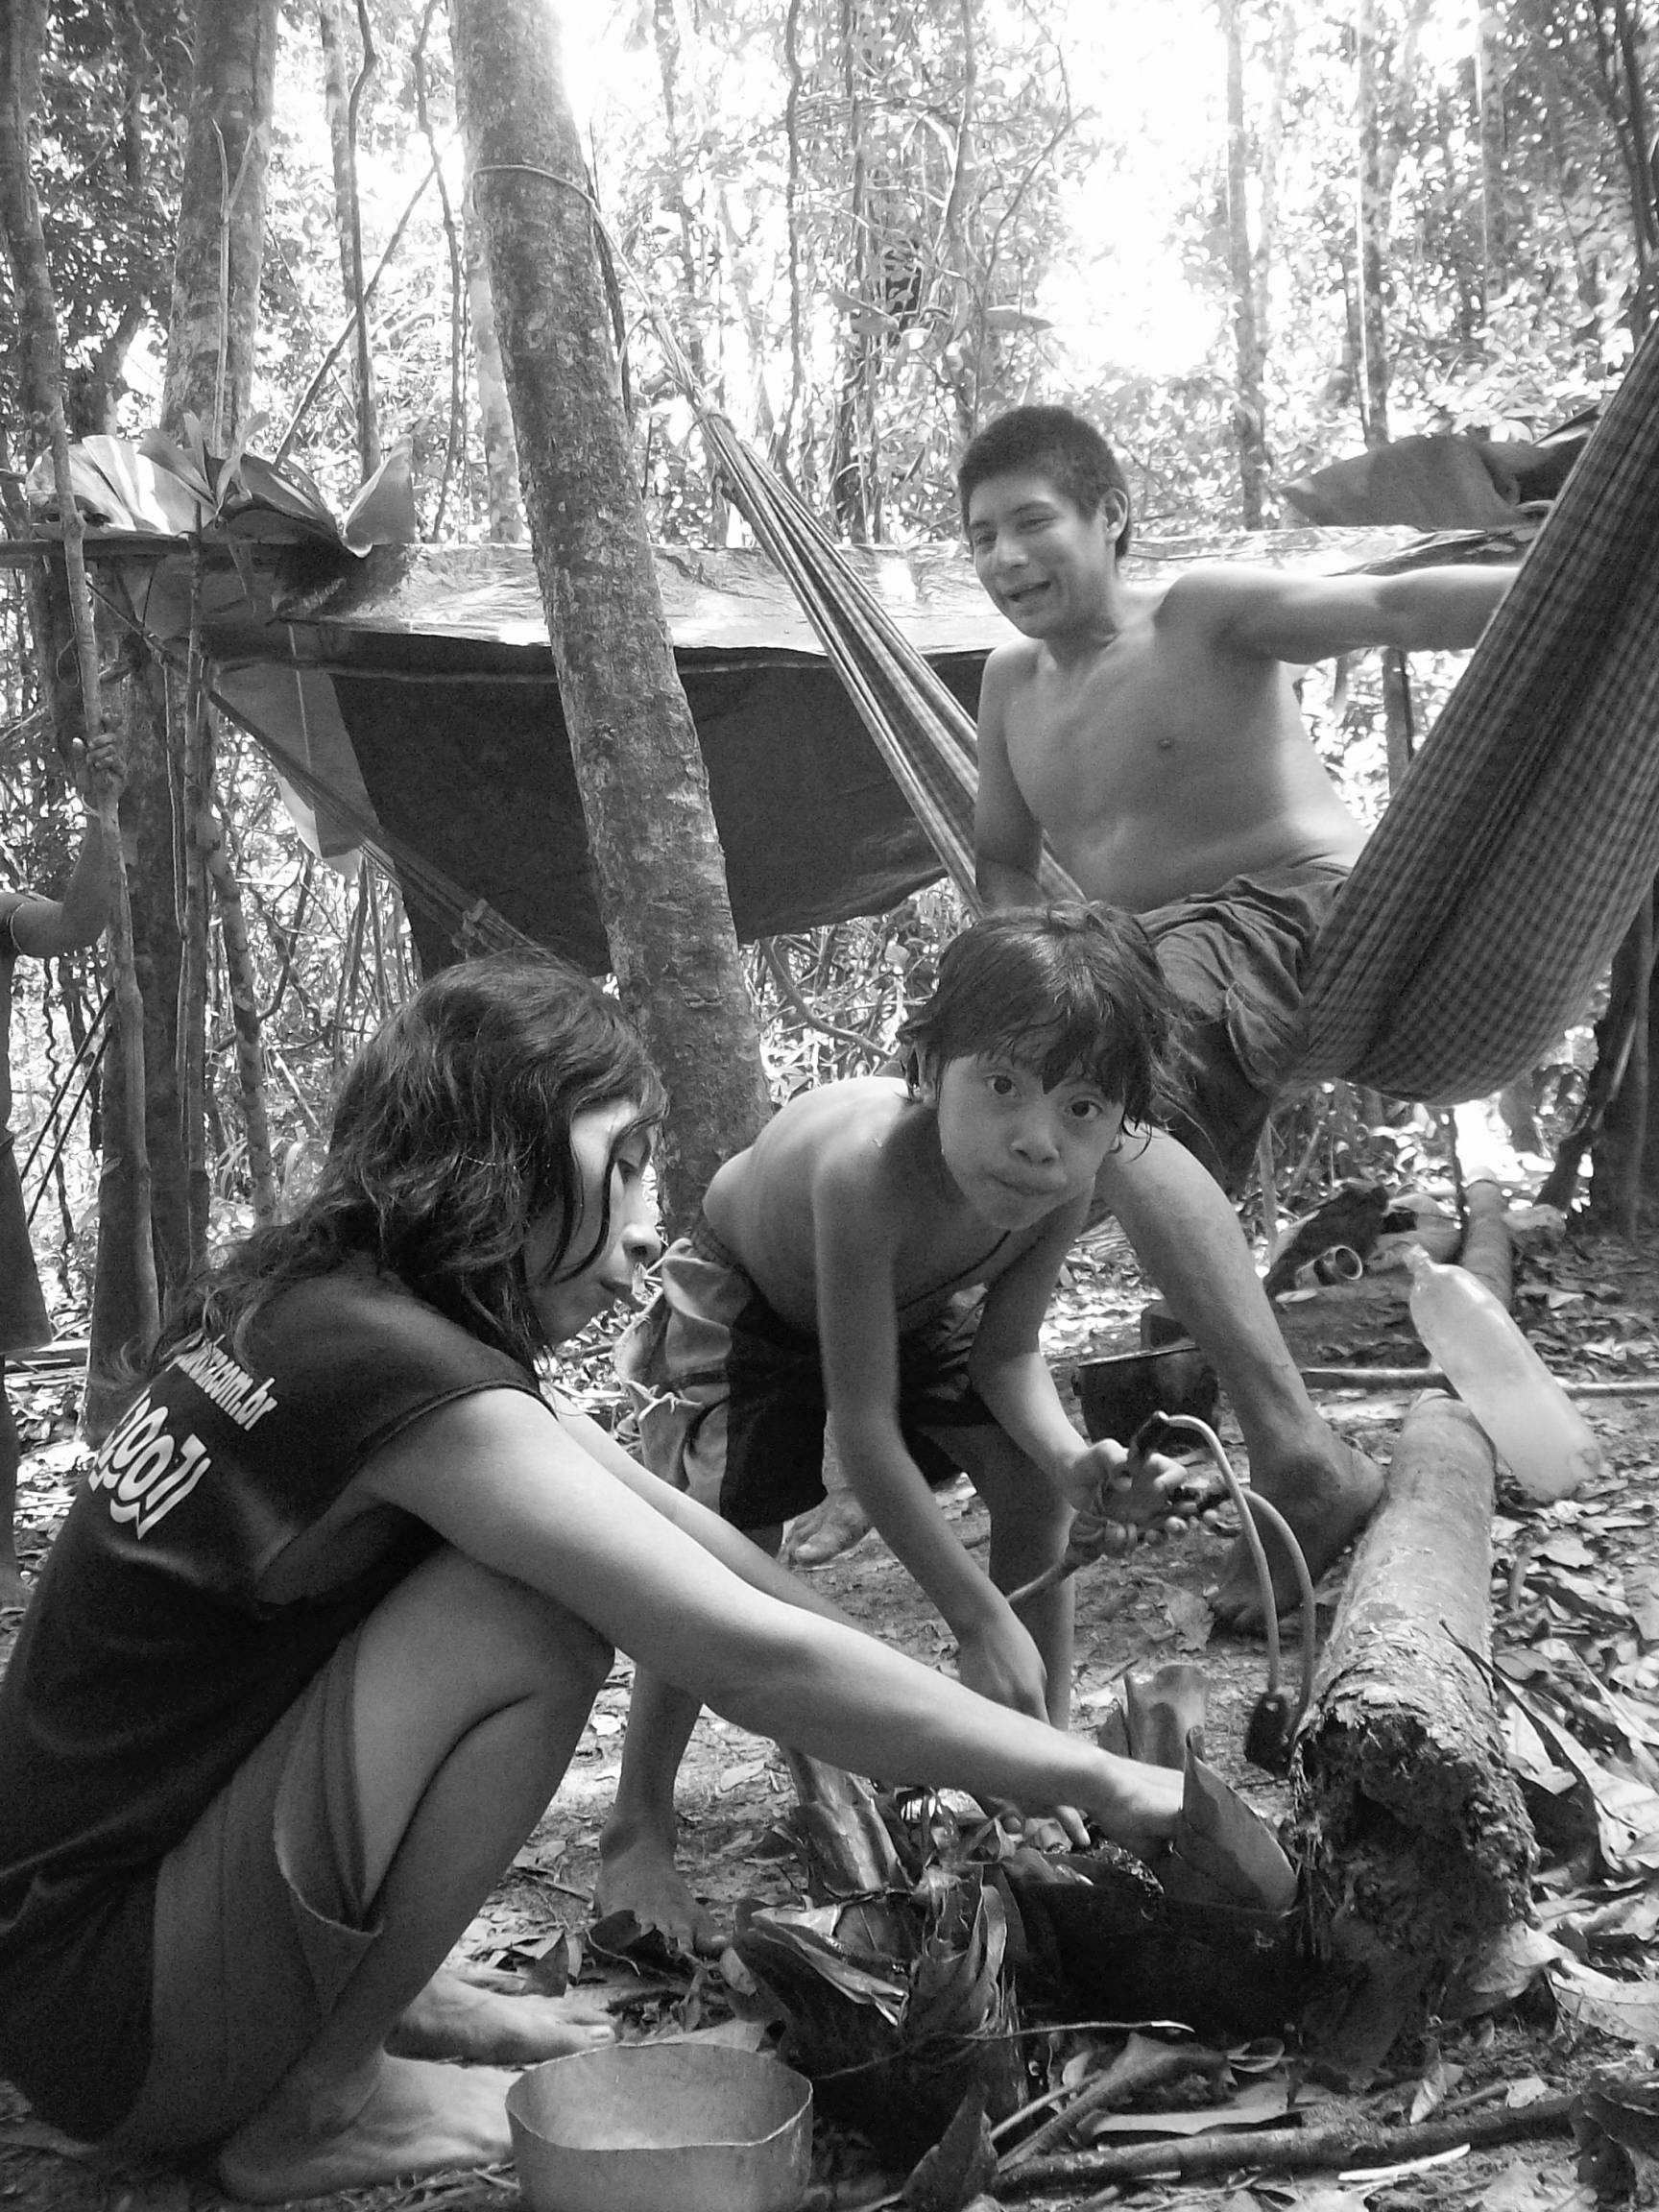
\includegraphics[width=\textwidth]{./imgs/100_4966}
%\caption{}
\end{figure}

\noindent Ideias que definem os Tupi como notáveis agricultores --- beneficiadores
de diversas espécies de mandioca, lavradores aptos ao cultivo das mais
variadas culturas, da batata"-doce ao fumo, passando pelo cará, milho,
amendoim, banana, pimenta, algodão, urucum, jenipapos e até cabaças;
produtores de farinhas e beijus; cauins fermentados e doces, dentre
outros cultivos específicos --- de forma alguma se aplicam aos
Guajá\footnote{Para a relação entre os Tupi e a agricultura, ver os
  balanços de Laraia (1986) e Viveiros de Castro (1986).}. A eles, como
vimos em sua história e, por consequência, no seu leque de opções
culturais, só restaram a caça de animais selvagens e a coleta dos frutos
da floresta. A agricultura está em uma fase embrionária, e o resultado
efetivo da incorporação dessa atividade no ciclo de vida das pessoas só
deverá ser percebido de forma qualificada dentro de algumas décadas com
o passar de, ao menos, mais uma geração. Enquanto isso, a caça, como
sugeri até aqui, segue como fenômeno central. Em nome dela, muitas vezes
estão dispostos a empreender um colossal investimento físico,
psicológico e mesmo emocional, e todas as outras atividades (pesca,
coleta de mel e frutos) parecem tributárias da caça. Muitos
acontecimentos se desenrolam a partir da caça: extrair mel, coletar
frutos (pequi, cupuaçu, bacuri, bacaba, inajá, dentre outros) e até
mesmo \emph{trabalhar} com a Funai são atividades passíveis de ser
abandonadas ou transformadas em caçadas, ao menor surgimento de um
rastro, indicação de um sonho ou mesmo pela pura \emph{vontade} de comer
determinada presa, como veremos mais adiante. O objetivo desse capítulo
é discutir os aspectos mais técnicos, psicológicos e econômicos das
atividades de caça e explorar o que seria, para os Guajá, essa atividade
--- como ela se inicia, o que é necessário para empreendê"-la e outras
questões semelhantes.

Forline (1997), que realizou um estudo de alocação de tempo das várias
atividades desempenhadas pelos Guajá, demonstra como a caça é, dentre
todas as atividades, aquela com que os Guajá gastam mais tempo em seus
dias, mesmo não sendo a carne de caça a principal fonte de nutrientes.
Embora cacem com eficiência diversos animais, os Guajá são especialistas
na captura de mamíferos arborícolas, em particular cinco espécies de
primatas: o capelão (\emph{Alouatta belzebul}), macaco cairara
(\emph{Cebus kaapor}), macaco cuxiú (\emph{Chiropotes satanus}),
macaco"-prego (\emph{Cebus apela}) e mão"-de"-ouro (\emph{Saimiri
sciuerus}). A técnica, que consiste em uma ``emboscada aérea'' dos
animais, ainda contemplaria a captura de quatis, ouriços"-caixeiros, e
preguiças\footnote{Tal como ocorre com outros animais que não são
  consumidos (ou são pouquissimamente consumidos), como a capivara e o
  tamanduá, as preguiças são abatidas sempre que os Guajá o conseguem.}.
A pesca sempre foi tradicionalmente uma atividade residual, uma vez que
os Guajá sempre viveram longe dos cursos de grandes rios, não possuíam
canoa, tampouco uma técnica apurada para a captura de peixes. Tal como
os Parakanã ocidentais, cujas proteínas ingeridas até o contato eram
oriundas basicamente da caça, os Guajá também, durante o período
pré"-contato, quando viviam na floresta, consumiam muito pouco peixe;
passaram a consumi"-los com mais frequência após sua redução aos postos
da Funai (inclusive com o auxílio de linhas, anzóis e tarrafas
fornecidos pela administração do posto). Mesmo ``bater timbó'', como
fazem hoje, aprenderam com os integrantes das primeiras frentes de
atração. Embora os peixes não figurassem no topo das preferências
alimentares, os rios e igarapés abasteciam as pessoas com a carne de uma
espécie jacaré (\emph{jakarea}) e de poraquês (\emph{manakya}). Além
desses, alguns quelônios como tartarugas e capiningas (\emph{Trachemys
adiutrix}) são muito apreciados. Em geral, os peixes eram capturados com
timbó ou flechas no auge da estação seca.

Com essa breve introdução, pretendo apresentar neste e no próximo
capítulo o rendimento ontológico da caça no universo guajá. Mulheres que
caçam, flechas que ganham vida, xerimbabos que guiam os humanos no mato,
além das sortes e azares dessa atividade que, mais do que isso, é a
definição da própria vida para essas pessoas. Veremos como a caça Guajá
tem como resultado um profundo manejo de espécies silvestres, em que o
fato de não matarem os filhotes e os soltarem em sua idade jovem; o
respeito ao hábito das espécies, escolhendo apenas algumas horas para os
abater; e não destruírem árvores ``duras'' (\emph{ira hatỹma'a}
``madeira dura''), lembrando"-se de que são elas os verdadeiros
\emph{habitats} dos animais (em oposição às árvores finas e moles,
\emph{ira memeka}, ``madeira mole'') demonstram não só um profundo
conhecimento bioecológico, bem como constitui, de muitas maneiras, uma
manejo particular sobre o ambiente, como veremos.

\section{Caçando com as mulheres}

Lembro"-me, no ano de 2007, da primeira vez que fui convidado a
acompanhar um pequeno grupo em uma caçada simples, de um único dia. Por
ser uma caçada de pacas e cotias, saímos por volta das sete horas da
manhã (um pouco mais tarde do que se fosse uma caçada de macacos) e
voltamos um pouco antes do anoitecer. Era um grupo pequeno. Comigo,
contávamos cinco: um casal (Wirahoa e Ajruhua), Juxa'a (o filho mais
velho da mulher, com cerca de 16 anos) e o velho Takya. Ainda levamos
duas cadelas, fundamentais para rastrear pequenos animais. E Ajruhua
levou seu \emph{kwixua} (cuxiú) de criação, empoleirado em sua cabeça e
que pulava de pessoa em pessoa, de galho em galho, e retornava às
cabeças à medida que caminhávamos.

Logo no início, percebi algo que seria recorrente a todas as caçadas que
eu iria presenciar: o fato de, se houver uma mulher adulta compondo o
grupo, toda a comunicação com os cães é feita por ela. Seus gritos
agudos são o sinal para que os cachorros, de longe, não parem de farejar
e respondam aonde estão. Os cães são delas! Durante todo o tempo, as
mulheres chamam pelos cães e eles, de longe, latem respondendo. E assim
segue, até que se ouve um latido mais forte, pontuado por rugidos,
acusando que encontraram a presa procurada. Nesse dia, após algumas
horas de caminhada, as cadelas rastrearam uma cotia que, poucos metros à
frente, se enfiara em um buraco. O terreno, muito acidentado, das serras
que compõem os territórios Guajá é formado por uma rede de buracos
feitos por tatus, pacas e cotias; muitos dos quais, ocultos, e que podem
ser chamados, como vimos, de \emph{akuti} \emph{rakwaha} (o ``domínio da
cotia'') --- buracos e troncos de árvores apodrecidos, os ``ocos de pau'',
que só um olhar especializado pode reconhecer. Ao encontrarem o
esconderijo em que a cotia se embrenhara, os homens começaram um
trabalho de escavação tão fundamental para a captura de cotias quanto de
pacas e tatus (durante o dia) --- para isso utilizam cavadeiras fornecidas
pela Funai. Em um período de quatro horas e em um raio de cinco metros
quadrados foram escavados sete buracos, alguns bem profundos.

Enquanto o jovem Juxa'a e o experiente Wirahoa escavavam as galerias
subterrâneas atrás do astuto roedor, quem indicava onde fazê"-lo ---
ouvindo a movimentação da pequena presa, se alinhando de barriga ao chão
e enfiando a mão nas fendas aberta --- era a mulher, Ajruhua. A cotia não
se entregou facilmente: encurralada no final, após fugir pelo
subterrâneo e ser reencontrada através de um novo buraco escavado pelos
homens, o animal, mesmo sem saída, conseguiu se enfiar na terra de tal
forma que não havia braços ou varas longas o suficiente para alcançá"-lo.
Nessa hora, Wirahoa junta alguns pedaços de palha seca de açaí
(\emph{jahara}), pega em seu mocó o isqueiro com que o presenteei
semanas antes, ateia fogo nas palhas e, junto com Ajruhua, abana e
assopra a fumaça tóxica para dentro do buraco. Essa fumaça ``envenenará''
a cotia, ele explicou, e a deixará bem ``mole''. E foi isso o que
aconteceu. Minutos depois de o buraco estar repleto de fumaça, a mulher
conseguiu apanhar a cotia pelo pescoço --- que saiu se debatendo com muita
força. Uma vez fora do buraco, Ajruhua a domou, segurando as patas
inferiores com bastante firmeza, enquanto que, com a outra mão, apertava
a garganta até que o animal morresse por uma asfixia final. Enquanto
isso, seu marido e filho estavam calmamente conversando e se limpando;
cansados e aliviados.

Mataram a cotia sem disparar um tiro ou flecha sequer. E o animal morreu
pelas mãos de uma mulher: fato muito corriqueiro, como pude, depois,
constatar. Nessa ocasião, percebi (o que também é recorrente) que as
mulheres não estão ali como ``damas de companhia'', como se as caçadas
fossem algo exclusivo de um apartado universo masculino. As mulheres
Guajá problematizam a ideia de caçar como algo do universo masculino, ou
um fenômeno fortuito, caso os homens não estejam presentes, como na
descrição de Lima sobre a participação eventual das mulheres nas caçadas
de porcos dos Yudjá (1996, p.22). Ao contrário, aqui elas muitas vezes
não só propõem as caçadas, como podem andar na vanguarda de um grupo,
destacadas na frente, indicando para onde ir, comunicando"-se com os
cachorros, rastreando fezes, urinas, pegadas, penas; enfim, todos os
tipos de vestígios (\emph{ipopora}) que devem ser sequenciados para que
haja uma caçada bem sucedida. Ajruhua é uma dessas mulheres. Seu marido,
Wirahoa, em 2007 era o melhor caçador da aldeia Juriti (em termos
absolutos, Wirahoa era o homem que trazia as maiores quantidades de
carne para casa). Porém quando caçam juntos, durante todo o tempo ele a
consulta sobre os caminhos a seguir e, muitas vezes, ela enxerga
possibilidades que ele não havia percebido. Como da vez em que ela
insistiu para andarmos um pouco mais, antes de desistirmos de uma vara
de porcos que, segundo muitos, já estava longe. E eis que encontramos os
porcos, após poucas horas de caminhada adiante. Enfim, ela tinha razão!

O fato de Ajruhua ser oito anos mais velha do que Wirahoa (ele tinha 29
anos em 2007, e ela, 36) pode ser um fator a se levar em conta; porém,
outros casais com idades próximas dividem com maior ou menor intensidade
o mesmo interesse pela caça: cada um de sua forma. Em uma tarefa
considerada universalmente masculina, a caça, inserida em um universo
como este --- em que predar é o centro da vida, e não uma atividade a mais
--- às mulheres só resta se juntar a seus irmãos, pais, maridos e
cunhados. Elas participam de todo o processo da caçada e podem,
inclusive, sair sozinhas a caçar (uma mãe e sua filha adulta, por
exemplo), principalmente cotias e pacas. Não é raro partirem de casa com
facões e machados e retornarem à aldeia com uma bela refeição e, ao
mesmo tempo, seus homens chegarem da mata, mas com as mãos vazias.

As mulheres desde muito jovens andam incansavelmente acompanhando também
seus namorados. Jovens namoradas, por serem alvo de muito ciúme da parte
de seus companheiros, não costumam ser deixadas sozinhas na aldeia
enquanto eles estão caçando. Elas, desde muito jovem, carregam seus
irmãos de colo ao acompanhar pais ou irmãos e, quando adultas, carregam
seus filhos junto com pesados machados, cavadeiras, facões e outros
instrumentos de metal. As mulheres ainda precisam dar conta dos
mosquitos e outros insetos (como mutucas e moscas) que, principalmente
na estação chuvosa, abusam da delicada pele dos bebês. Para afugentar
essas ameaças, cada uma delas porta um abanador (\emph{tata maka}), tal
como leques, que passam abanando sobre os filhos na tipoia durante toda
a caminhada. O leque, a tipoia, a saia, e o animal de criação
(\emph{haima}) adornando a cabeça compõem a indumentária feminina
durante as longas caminhadas e caçadas.

Durante caçadas coletivas, ao encurralar algum animal, as mulheres podem
dispor de uma das flechas do marido. Elas as enfiam no buraco ou entre
as árvores, no intuito de ferir ou acuar a presa; se proteger ou ameaçar
algum animal; e não há restrições quanto a uma mulher tocar nos arcos ou
flechas de seus maridos. Muitas vezes, durante as caminhadas, se os
homens estão muito carregados, suas esposas levam para eles seus feixes
de flecha, arcos ou espingardas. Ao final de caçadas em que eu os
acompanhava, as mulheres gostavam de posar para minhas fotos segurando
os arcos e espingardas de seus maridos, bem como as caças abatidas por
eles. Quando posavam, diziam em tom de brincadeira terem sido elas que
mataram aqueles animais. E se cerca de uma década atrás as mulheres
seguravam arcos e espingardas apenas para aliviar o peso dos homens, nos
últimos anos, pelo menos em uma das aldeias, mãe e filha passaram a
caçar com espingarda. Ao visitar pela última vez a aldeia Tiracambu, em
2014, alguns amigos relataram o fato de Ximirapia e Pinawãxika, mãe e
filha, respectivamente, estarem caçando com uma espingarda que estava
``sobrando'' na casa de uma das duas, o que, definitivamente, me parece
uma novidade nesse estilo de caça realizado pelas mulheres. Estariam
elas matando inclusive macacos, algo até então nunca experimentado. Além
disso, os Guajá relatam que em situações excepcionais mulheres
confeccionam e utilizam arcos e flechas. Este é o caso das duas mulheres
encontradas ``isoladas'' em 2015 (a finada Jakarewãja e Amakaria), que
tiveram que criar sozinhas o pequeno Wirahoa. No mato, uma delas
fabricava arcos e flechas, caçava com eles e ensinou o menino a caçar
até que ele pudesse fazê"-lo também.

É muito comum também as mulheres levarem às caçadas seus filhos com
idade de até dois anos. Levam"-nos na tipoia (\emph{imymy menẽha}), que
até o contato era feita com fibras das folhas tucumã, mas hoje se faz
com tecido. Muitas vezes, devido às longas distâncias percorridas com as
crianças na tipoia, uma mulher pode pedir a seu marido que carregue a
tipoia com a criança por algumas horas. Nesse caso, ela mesma carregará
a espingarda ou arco e flechas do marido, em uma cena atípica na
literatura sobre caça, eu diria. Muitas foram as vezes em que os vi
trocarem os pesos ``masculinos'' e ``femininos'' para aliviar o desgaste da
mulher. Uma hipótese, que goza de longa história na antropologia, de que
as mulheres não caçam pois estão ``constrangidas, sobrecarregadas, ou
imobilizadas presas aos cuidados infantis'' (Noss \& Hewlett, 2001,
p.1025), tal como apontada por alguns autores (Brightman 1996; Noss \&
Hewlett, 2001), também não se confirmaria aqui.

Não existem caçadas de que uma mulher não possa participar junto com seu
marido ou irmãos; é mesmo muito comum as meninas recém"-noivas (ou
``pegas'', como dizem todos) e que ainda moram na casa dos pais
acompanharem os homens com quem irão se casar. Quase sempre, as
primeiras carícias e descobertas do sexo são experimentadas nesses
passeios de caça. Mesmo na caça de queixadas --- a mais desgastante e
arriscada dentre todas, pois os homens são obrigados a se separar, saem
completamente dos caminhos e trilhas usuais, se embrenham entre espinhos
e por áreas fechadas da mata (e tudo isso correndo\ldots{} correndo muito) ---
as mulheres podem estar presentes, embora, nessas situações, elas não
corram tanto nem se embrenhem com vigor entre espinhos e por áreas
fechadas, tal como fazem os homens. Caso estejam na mata em companhia de
seus maridos (ou parentes do sexo masculino), as mulheres esperam em
algum local seguro; ou, se a caçada se estender por muitas horas,
simplesmente voltam à aldeia (sempre acompanhadas por algum homem
destacado para isso). Mesmo na caçada de porcos, em que dificilmente
elas participam diretamente da ação --- tal como fazem na captura de
outros animais ---, uma mulher pode ajudar seu grupo a rastrear os
queixadas e planejar estratégias de captura. Assim, de muitas maneiras
um casal pode ``andar junto'' (\emph{wata} \emph{pyry}) atrás de caça; e o
interesse de uma mulher por caçar é considerado mais que desejável, uma
vez que, como estamos vendo, durante muito tempo essa foi a ``principal''
atividade na vida das pessoas.

Para os Guajá, portanto, nada mais ``natural'' do que mulheres se
envolverem nas caçadas. A partilha de interesse de uma mulher por essa
atividade, quase sempre, só tem a acrescentar ao desempenho de seus
maridos. Tenho, por suposição, que os melhores caçadores geralmente
contam com uma ou mais esposas interessadas no assunto. Ou, em outras
palavras, o sucesso na caça será consideravelmente superior para um
homem quando a mulher se envolve, uma vez que ela entende como poucos as
artimanhas dessa arte. Ajruhua e Amỹ Pirahỹa, por exemplo, quando saíam
com um grupo grande --- formado por filhos, maridos, irmãs e cunhados ---,
eram constantemente consultadas por homens para expressar suas opiniões
e decisões a respeito de determinados ``rastros'' (penas, fezes, urinas,
pegadas, tudo o que compõe a ideia de \emph{ipopora}, ``rastro'') e os
caminhos a seguir. O mesmo pude ver na aldeia Tiracambu, onde um dos
homens que mais capturava, Maihuxa'a, tinha em sua esposa, Pakawãja, uma
grande companheira de caça, muito interessada no assunto, e o casal, tal
como Ajruhua e Wirahoa, participava de todo o processo de caçada, que
consiste basicamente em rastrear, cercar e abater.

Uma ideia genérica de mulheres indígenas como coletoras de frutos ou
produtoras de beiju não expressa o forte comprometimento que as Guajá
mantêm com a atividade de caça. Além disso, muito do que é coletado o é
feito pelos homens, principalmente a bacaba e o inajá, frutos que são
apanhados por pessoas que têm que subir em suas árvores e que muitas
vezes têm como resultado cortes e escoriações profundas. Pequi, babaçu,
bacuri e cupuaçu realmente são possíveis de ser colhidos por mulheres e
crianças, porém, na época da bacaba (entre desembro e março de anos
alternados), se não fossem os homens para apanhar os cachos, o consumo
da fruta não seria sequer metade do que é. Quero com isso defender que,
para os Guajá, a relação entre caça e coleta não está diretamente
condicionada aos sexos masculino e feminino, pelo que homens ``caçariam''
e mulheres ``coletariam'', tal como usualmente encontramos em textos sobre
grupos caçadores, passíveis porém de uma necessária crítica. Brightman,
por exemplo, argumenta que a generalização a respeito da ideia de
\emph{caça masculina} e \emph{coleta feminina}, tão difundida na
bibliografia etnológica a respeito de povos caçadores"-coletores,
obscurece variações específicas do modo de produção particular
encontradas em cada sociedade em particular, já que em muitos contextos
as caças menores são capturadas por ambos os sexos ou, em alguns casos,
preferencialmente por mulheres (Brightman, 1996, p. 689)\footnote{O
  trabalho em sociedades caçadoras e, mais especificamente, a
  contribuição das mulheres em caçadas é um tema bastante descrito na
  bibliografia acerca de povos caçadores"-coletores. Ver Brightman (1996)
  ou Noss and Hewlett (2001).}. Muito embora as mulheres não cacem como
homens --- uma vez que a diferença entre os sexos passa pela diferença
tecnológica: os homens utilizam armas; as mulheres, não ---, se aceitarmos
que as caças menores, junto com os capelães, representam a maior parte
da quantidade de proteínas consumida pelos Guajá (ver Forline, 1997),
podemos apontar que as mulheres são componentes fundamentais a essa
atividade, e não meras substitutas ou colaboradoras. E mesmo o argumento
tecnológico --- tão definitivo para dar conta das assimetrias entre homens
e mulheres na caça, em que mulheres não usam armas, ``\emph{Ce n'est pas
la chasse qui est interdite aux femmes, ce sont les armes}'' (Não é a
caça que é interdita às mulheres, mas as armas) (Tabet \emph{apud} Brigthman,
\emph{op. cit.}, p. 705 ), se nos basearmos pelas ``mulheres caçadoras'' que
vivem em isolamento ou por Ximirapia e Pinawãxika, mãe e filha da aldeia
Tiracambu que vêm caçando com espingarda, tal afirmativa parece não se
aplicar totalmente no caso Guajá.

%\textbf{Mostrar foto de Pinawxiká com sua espingarda}
\begin{figure}[H]
\centering
  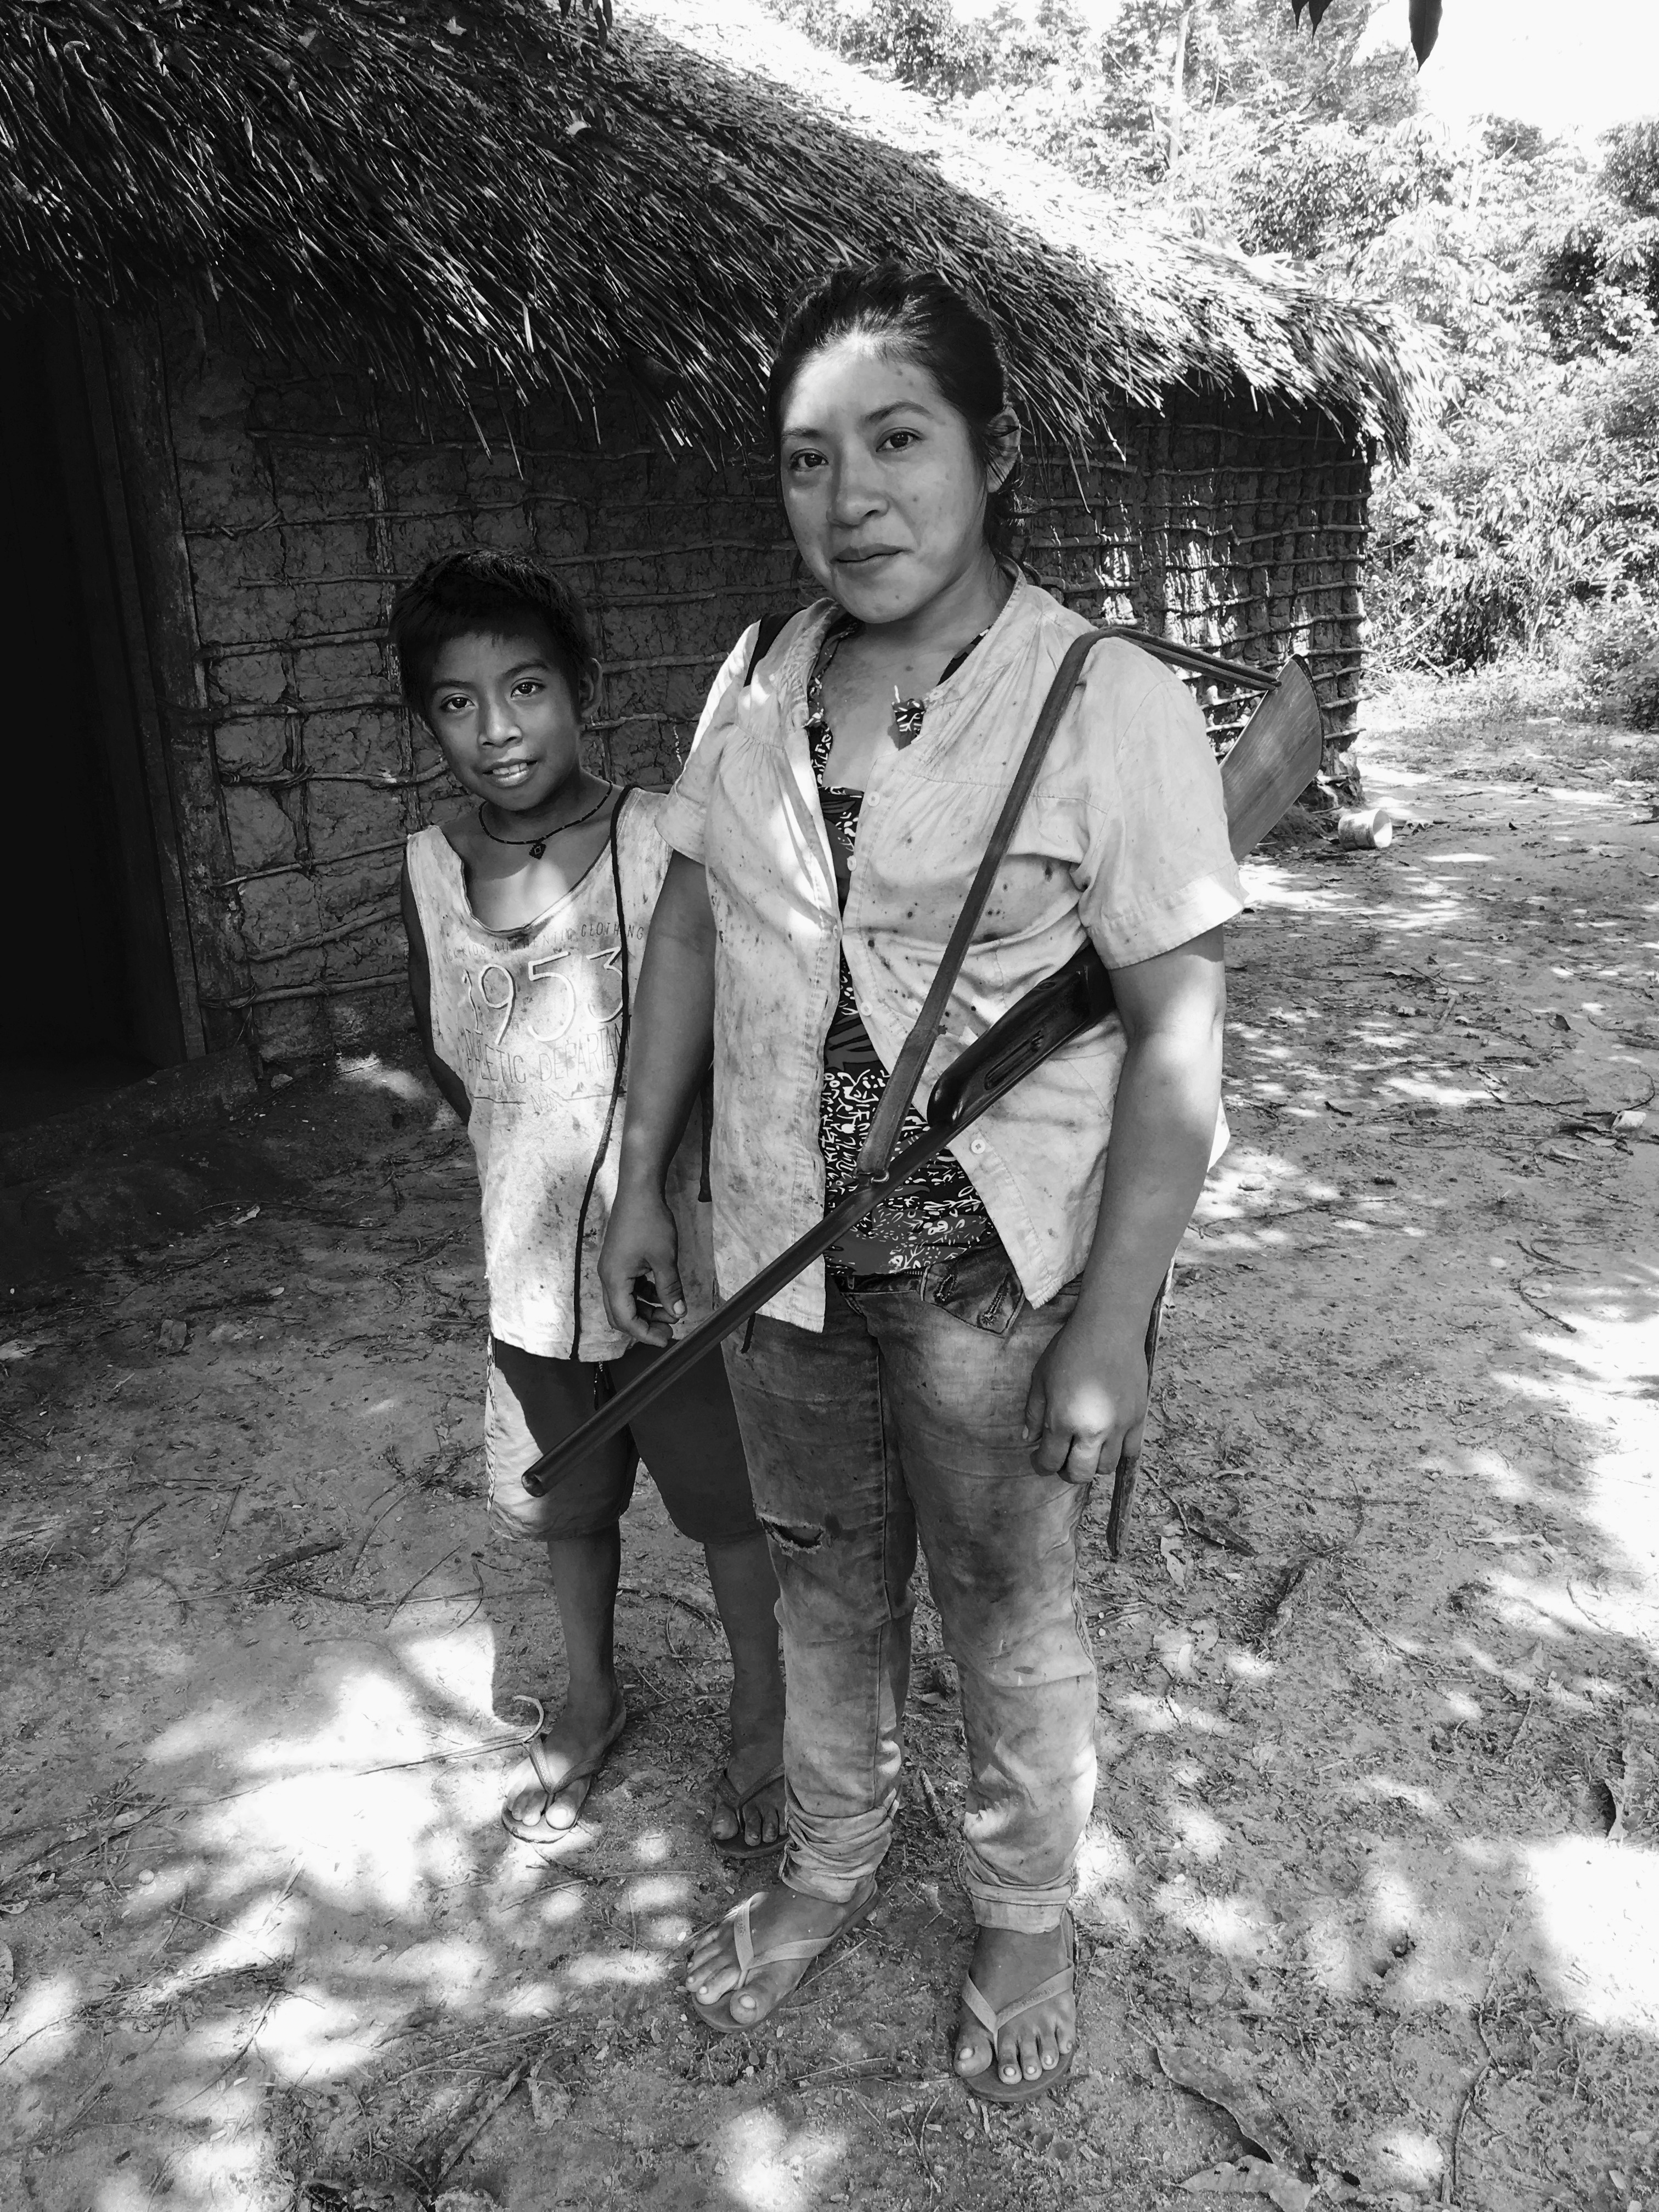
\includegraphics[width=\textwidth]{./imgs/IMG_4463}
\caption{Foto de Pinawxiká com sua espingarda}
\end{figure}

Por outro lado, em nenhum momento os Guajá defendem a floresta como um
local seguro e prazeroso para uma mulher permanecer só, pois, mesmo
sendo caçadoras, são sensíveis à violência natural da mata. Apesar de
não excluírem as mulheres das caçadas (sendo, inclusive, desejável que
participem --- como estamos vendo) e muito embora defendam a presença de
suas esposas, irmãs e filhas nessa atividade, os homens guardam cautela
quanto à relação mulheres"-mata. Mesmo sendo caçadoras (\emph{watama'a},
``caminhador'') elas são desencorajadas por seus maridos em algumas
situações. São"-lhes sempre lembrados os riscos de toparem com uma
onça"-pintada (pois as sussuaranas e onças"-pretas oferecem pouco perigo).

``Eu quero ver anta, veado, vamos andar"-caçar (\emph{wata}), meu
marido!?'', assim Wirahoa sintetizou"-me as chamadas de sua esposa para
irem caçar quase que diariamente. É uma atividade prazerosa para todos,
e as mulheres gostam (\emph{maparỹ}) da floresta como qualquer outro.
Porém, mesmo diante dos clamores exortativos femininos, os homens
guardam cautela à constante insistência delas para caçar, sejam
acompanhadas pelos homens ou por outras mulheres. A pronta resposta
masculina é, quase sempre, ``não vá, pois é perigoso, a onça te comerá!'',
ou outra coisa de ruim acontecerá. Em caso de encontro com as
onças"-pintadas (\emph{jawaruhua} ou \emph{jawarapeperemuhũa}), os homens
lembram que conseguem se defender e correr melhor do que as mulheres.
Além disso, Pakwa'ĩa, uma mulher, me explicou certa vez que as onças
preferem comer a carne feminina à masculina, bem como uma criança a um
adulto. Por essas e outras razões, uma mulher deve caçar de preferência
junto com o marido (\emph{wata} \emph{pyry}), embora isso não ocorra na
prática com a mesma frequência que é relatada no discurso dos homens.
Devo acrescentar que o ``fator cachorro'', como veremos neste capítulo, é
fundamental para que as mulheres tenham autonomia suficiente para entrar
sozinhas na mata; não só porque os cães espantam as onças e outro
animais perigosos --- proporcionando segurança ---, como também porque
facilitam, em muito, o trabalho de captura de roedores e tatus que, ao
lado dos quelônios, são animais facilmente capturados e abatidos por
mulheres.

O fato de a floresta ser supostamente mais perigosa para uma mulher que
para um homem parece ser, ao menos aparentemente, algo com que todos
concordam; pois os homens, pelo fato de possuir armas, conseguir subir
em árvores, aguentar mais peso, dentre outras vantagens técnicas,
seriam, pelo menos dizem os Guajá, mais preparados para enfrentar a
mata. É interessante notar que, apesar da ideia de ser a floresta um
local perigoso para as mulheres --- e do fato de os homens em geral se
utilizarem de armas, e as mulheres não ---, em nenhum momento homens
defendem que a caça é uma atividade \emph{masculina} em oposição a outra
atividade (como a coleta) que seria \emph{feminina}. Evocando aqui a
crítica de Marilyn Strathern (1980), o próprio par referente à
\emph{esfera doméstica}, representada pelos animais de criação ---
filhotes cujo manejo da vida depende das mulheres ---, e a \emph{esfera
selvagem} concebida quanto a animais de caça, em que os homens são
agentes privilegiados dessa relação, deve ser visto com cautela, uma vez
que os animais de criação que acompanham mulheres à mata ali estão não
apenas como adereços para o corpo (como já tentaram sugerir). Em conexão
com suas donas, macacos pregos e cairara, atentos às caminhadas, podem
alertar com assobios e gritos sobre cobras e aranhas venenosas durante o
trajeto (Diniz 2014, p.65). O mesmo pode ser visto --- como observaremos
mais à frente --- com os cachorros. Desde a introdução desses animais nas
atividades de caça, as mulheres passaram a andar com mais segurança no
mato, com menos ameaça de serem atacadas por onça, e grupos de mulheres
com seus cachorros costumam ser muito eficientes em caçadas. Se a
floresta é um local perigoso para as mulheres, como os homens costumavam
me dizer, com os cães os riscos são amenizados. Os animais de criação
aqui, longe de serem exclusivos da aldeia (\emph{esfera doméstica}) em
oposição à pura predação de uma suposta \emph{esfera selvagem}, são
importantes justamente na mata.

Sabemos há algum tempo que as diferenças entre mulheres e homens não
estão necessariamente baseadas na divisão entre natureza e cultura,
muito menos podem ser diretamente correlacionadas a uma oposição entre
``doméstico'' e ``selvagem'' (Strathern 1980). Como já pontuado aqui, a
questão de homens desaconselharem mulheres a entrar sozinhas na floresta
e o fato de a caça acontecer na mata não podem ser reduzidos à ideia de
que a caça seja uma atividade masculina por excelência, embora seja
bastante desejável pelo mulherio (\emph{awa wahykera}) que os homens
cacem para as esposas, e muito do que as mais velhas almejam ao se casar
com homens mais jovens é que eles caçarão para elas. Porém, nem por isso
a caça é pensada como uma atividade exclusivamente masculina.

Para os Guajá, o selvagem (\emph{ka'a}) e o doméstico (\emph{tipa}) não
parecem encontrar ecos automáticos em outras oposições (supostamente)
manifestadas como masculino e feminino; humanidade e animalidade. Por
isso, o problema aqui --- mais uma vez --- repousa na imposição de uma
dicotomia analítica a situações em que ela não é apropriada (Strathern
1988, p.20). A ``animalidade'' de um animal de criação, muito
provavelmente, em nada se conecta à animalidade de um animal selvagem
que será caçado. Diferentes modos de relação recortam os animais em duas
categorias distintas entre si: \emph{hanima} (``meu animal de criação'')
e \emph{ma'amijara} ou apenas \emph{ma'a} (``presa'', ``caça'',
``bicho''). Um animal que é tratado por presa nunca será de criação, e
os filhotes capturados dessas presas (apenas os muito pequenos)
raramente são vistos como ``caças'' (\emph{ma'amijara}). Os filhotes
capturados devem ser muito pequenos, pois aqueles um pouco maiores são
difíceis de amansar e ainda poderão, em algum momento, se vingar da
morte de seus pais, atacando principalmente as crianças. Filhotes de
macacos, queixadas, caititus, esquilos quatipuru, cotias, papagaios,
quatis e macacos"-da"-noite são criados na aldeia, e quase todos
acompanham suas donas em caçadas e incursões pela floresta. O fato de
animais serem domesticados é o que, de muitas maneiras, colabora para
que as mulheres cacem mais, com mais vigor e qualidade, e mais ainda as
remete --- com mais segurança, pois esse é um ponto importante aqui --- para
a floresta.

\section{A vontade de ``querer ver''}\label{a-vontade-de-querer-ver}

Em sua teoria sobre a caça, os Guajá defendem que a vontade de matar um
animal específico é fundamental a uma caçada produtiva. Certa vez, após
passar um dia na floresta acompanhando Pira'ima'ã, voltamos para casa
com as mãos vazias, reflexo do péssimo dia de caçada. Em nossa caminhada
de retorno, Pira'ima'ã comentou: \emph{axaku'uhy wari ikaha}!, sentença
que pode ser traduzida por algo como ``estou com muita vontade de matar
capelães!'' Isto indicava que o fato de não os ter matado poderia,
inclusive, lhe fazer mal, já que aumentava cada dia mais essa vontade,
que é chamada \emph{xaku'uhy} e permite uma tradução como ``querer ver''.

De acordo com Magalhães (com. pess.), -\emph{xaku'uhy} é um verbo que
pode ser traduzido grosseiramente por ``sentir falta'' ou ``ter saudade''.
Mas, analiticamente, ele pode ser segmentado em três partes: \emph{xak}
``ver''; -\emph{u'u} um morfema encontrado em poucas palavras e que
significa ``desejar'', ``querer''; e -\emph{hy} um sufixo que indica a maior
intensidade com que é empregada a palavra (por exemplo: \emph{i'ĩ}
significa ``ele falou'' e \emph{i'ĩ-hy} ``ele ralhou'' ou ``falou de maneira
mais forte''). Dessa forma, ``ver (\emph{xak})-querer (-\emph{u'u})'', isto
é, ``querer ver'', parece uma tradução satisfatória. No caso em questão,
Pira'ima'ã estava com vontade (ou ``saudade'') de comer capelães. Isso
pode ser bom, pois promove novas caçadas; mas também pode ser ruim, pois
a frustração acarreta problemas.

Por exemplo, em uma caçada há sempre uma predisposição para matar
animais movida por uma vontade que não será saudável se for frustrada.
Caso seja frustrada, deve ser sanada. Tal vontade pode ser produzida por
algum evento: como um sonho, uma conversa, o conhecimento de um novo
rastro e mesmo, obviamente, a fome (\emph{hajamyhỹ}, ``estou com
fome''). As duas ou três refeições que os Guajá gostam de fazer em um
dia são completadas por ceias menores, compostas por frutos, pedaços de
carne, mel com farinha, hidromel, iguarias como fígados, língua e
cérebro de alguns animais, bolachas e toda sorte de alimentos que
estiverem ao alcance da mão. As crianças são capazes de passar os dias
comendo, e são justamente elas e as mulheres que mais exigem comida. Em
um belo relato sobre os Aikewara, Tupis do leste do Pará, Calheiros
afirma que ``um caçador, se for perguntado sobre os motivos que o levam
a abandonar a sua rede e partir para a mata em busca de caças,
responderá indicando uma mulher que vive junto dele: os solteiros dirão
que caçam para suas mães e irmãs mais novas, os casados, que caçam para
suas mulheres e filhas'' (2014 p. 177); e essa ``fome'', destaca
Calheiros, mobiliza as comunidades e mantém os homens em movimento. Nas
aldeias Guajá, crianças famintas ficam muito zangadas e, por isso, podem
brigar entre si, chorar de forma desmedida, bater em xerimbabos e, mais
comum do que possa parecer, arrancar os próprios cabelos em desespero.
Os pais sempre que saíam para caçar diziam a mim, mesmo em português,
``tenho que caçar, as crianças estão com fome!'' Por isso, a
``vontade'', para ser aplacada, quase sempre nem será a própria vontade
do caçador, mas a dele e a dos outros relacionados a si (mulheres,
filhos), o seu \emph{pessoal}, para evocar a tradução dos Yudjá (Lima
2005 p. 110).

Uma caçada frustrada (perdida, não realizada) pode criar um desejo de
matar ainda maior, deixando os homens transtornados (\emph{waky}
``loucos''), com raiva (\emph{imahy}) acumulada, o que os obriga a ir para
a floresta muitas vezes sozinhos e só voltarem quando a raiva tiver
passado --- o que só acontecerá após matarem o máximo de animais que
conseguirem. Por outro lado, essa vontade \emph{xaku'uhy} (``querer ver'')
é umas das características que mobiliza os Guajá para a caça. A relação
entre vontade e ação não tem um centro fixo de irradiação. Não há uma
palavra de ordem que os mobilize para a caça ou qualquer outra
atividade. E os eventos podem ocorrer como que por ``vontade própria''.

Certa vez, após comermos muitos inajás, fiquei curioso para experimentar
o coco desse fruto, pois, como se sabe, do inajá consumimos somente o
fruto --- cozido, assado ou na forma de mingau --- e seu coco é normalmente
descartado. Alguns me disseram que não comiam o coco do inajá pois a
casca, além de muito dura e difícil de arrancar, escondia um coco muito
pequeno, cujo esforço não valeria a pena. Nessa manhã, talvez por falta
do que fazer, peguei emprestada a cabeça de um machado e um toco de pau
a fim de abrir alguns cocos de inajá que abarrotavam o chão, em volta de
um moquém, onde haviam sido cozidos. Ajudado por alguns meninos, comecei
a atividade. Assim que abri o primeiro coco, logo me decepcionei,
constatando que era preciso um esforço muito grande para retirar a casca
e que o resultado era uma noz pequena e sem gosto, quando as pessoas me
disseram em tom de galhofa: \emph{kwaj kĩ mehẽ!!!} (``tá vendo!!!?/não
disse!!!?''). De todo modo, prossegui na operação, abrindo mais cocos ---
mais por esporte do que por outra razão. Logo vi que estava sendo
acompanhado por alguns garotos que faziam o mesmo. Minutos depois, boa
parte das crianças da aldeia estava espalhada quebrando cocos de inajá
para comer. Em seguida apareceu Pira'ima'ã, querendo amolar meu machado.
E passou, ele mesmo, a quebrar cocos de inajá; chegou também sua mulher,
Pakwa'ĩa, e instantes depois, seu pai, o velho Pirama'ã, além de outras
pessoas. Em menos de meia hora, um exercício inútil movido por uma tola
curiosidade havia se transformado em uma ocupação que tomou dezenas de
pessoas da aldeia Juriti. Da mesma maneira, muitas vezes os desejos,
inclusive por uma caçada, podem se iniciar desta forma, meio que por
contágio.

Por isso, há uma grande dificuldade por parte dos funcionários da Funai
de arregimentá"-los para os trabalhos da roça, pois palavras de mando não
surtem o mesmo efeito que uma epidemia de vontades. É comum os
funcionários marcarem uma colheita ou plantio para o dia seguinte e, na
hora em que estão indo para a roça alguém anunciar um novo rastro de
porcos ou um grupo de capelães; e então, todos abandonarem o ``trabalho'',
deixando os funcionários sozinhos na roça. Em outras diversas situações,
quando um trabalho na roça ou no pomar não estava marcado, as pessoas
muitas vezes se encaminhavam uma a uma (tal como no episódio do inajá)
para trabalhar, deixando os funcionários do posto sem entender, já que
isso não estava previamente ``combinado'', isto é, não tinha havido
palavras de mando. Simplesmente os Guajá começaram. Não se trata somente
de a roça ser algo menos interessante do que a caça (o que é fato), mas
a forma como se inicia uma atividade nem sempre é escolhida por todos.
Simplesmente começam, como se fossem tomados por uma grande vontade
mobilizadora, que defendo aqui ser o \emph{xaku'uhy} (``querer ver''),
importante tanto para a caça quanto para a vida, de maneira geral.

Viveiros de Castro --- como lembrou Fausto --- ``descreveu com elegância o
caráter epidêmico das ações coletivas em uma sociedade sem chefia''
(Fausto, \emph{op. cit.}, p. 275):

\begin{quote}
\emph{Fruto menos de deliberações formais ou tomada de decisão de alguns em
nomes dos outros, os atos concertam"-se por um processo social de
contágio. Ninguém diz a outrem o que deve fazer, mas sugere o que ele
próprio fará. (\ldots{}) é preciso, contudo, que alguém dê início à ação,
tirando da inércia as disposições}.
\end{quote}

Fausto comenta como tal característica se presta à guerra Parakanã
(Fausto, \emph{op. cit}., p. 275), e Viveiros de Castro, como tal ``caráter
desordenado e paulatino'', rege boa parte das ações Araweté (Viveiros de
Castro, 1986, p. 300). A partir de noções específicas sobre as relações
humanas, tal como \emph{tenetãmõ}, ``o que segue à frente'', e
\emph{tãnã}, ``o dono da aldeia'', Viveiros de Castro observa que ``toda e
qualquer empresa coletiva Araweté supõe um \emph{tenetãmõ}'', e ``uma
coisa não começa se não houver alguém em particular que a comece''
(\emph{idem}). O cognato Parakanã para o \emph{tenetãmõ} dos Araweté é
\emph{tenotara}; na guerra, eram eles que iam à frente, eram os
primeiros, dotados de uma grande capacidade exortativa (Fausto, op.
cit., p. 276). A ideia de \emph{tãnã} Araweté, que está baseada na
aldeia, no componente espacial, encontra entre os Guajá o termo
\emph{tamỹa}. Por isso, aludem para o fato de \emph{Maira} ser um
\emph{iwa} \emph{tamỹa,} um líder nas aldeias celeste.

Se o problema da liderança (mais do que chefia), como parece ser, é este
de fazer aparecer um coletivo em que o líder é aquele que inicia,
coordena ou mesmo captura uma ação (Sztutman 2012, p.316), os Guajá
lembram que o \emph{chefe} (sendo esta uma glosa indígena) é aquele que
``puxa'' uma ação coletiva. Uma ideia importante na política é aquilo
que traduzem para o português por ``puxar''. \emph{Myty}, ``puxar'',
seria a principal atribuição de um \emph{tamỹa} (o \emph{chefe}; que vai
na frente). \emph{Myty ipamẽ} pode ser traduzido por ``puxando juntos um
ao outro'', e os trabalhos na roça, caçadas e outros movimentos são
sempre assim concebidos. Para todas as atividades, além de outros níveis
da própria existência, as figuras de \emph{tamỹa} ou \emph{xipa}
\emph{tamỹa} (o ``velho/pai que lidera'') são sempre evocadas. E apesar
da complexa e (muitas vezes) categórica diferença entre ``chefia'' e
``liderança'', tão bem documentada em trabalhos como o de Sztutman
(2012), a glosa guajá para essa figura do líder --- o que toma a frente e
mobiliza um coletivo --- é sempre \emph{chefe}, e mais recentemente
\emph{cacique}, como é o caso de jovens chefes de família que acumulam
uma função no diálogo interétnico contemporâneo que, como bem mostrou
Yokoi (2014) em sua dissertação sobre política Guajá, ainda estamos
vendo para onde levará a se mover a figura do \emph{cacique}. Quando
todos os chefes de família se pensam e são pensados como \emph{tamỹa},
em situações de tradução como nas reuniões com a Funai ou Sesai, muitas
vezes os jovens \emph{caciques} dizem que não conseguem despertar o
interesse de toda uma aldeia para uma atividade previamente acordada com
o órgão; quando muito, eles o conseguem com suas famílias e aliados.
Certa vez, o jovem Manã, da aldeia \emph{Awá}, explicitou tal problema
em uma conversa de ``líderes'' (leia"-se jovens interlocutores) com a
equipe de índios isolados da \versal{FUNAI}, lembrando que tudo aquilo que eles
estavam combinando ali (mudança no jeito de fazer as roças, usos das
torneiras da aldeia dentre outras importantes decisões) de nada
adiantaria, pois quando ele voltasse para casa o combinado funcionaria
melhor para seu grupo de parentes e amigos do que para os outros. A
profusão das figuras de \emph{chefia} nas aldeias maiores também é
discutida por Yokoi, aludindo à conhecida diversidade de grupos locais
nos diversos territórios (\emph{hakwaha}), antes do contato. Com isso,
\emph{tãmya}, segundo o autor, ``poderia ser considerado como o dono do
espaço de circulação de seu grupo, tendo em vista a mobilidade Guajá em
seus \emph{hakwaha}. (\ldots{}) Como a aldeia Awá é uma reunião de vários
grupos dispersos podemos encontrar muitos \emph{tãmy} por lá, diria que
(\emph{tãmy}) são todos os homens com mais de trinta anos e que de certa
maneira são ativos na vida pública da aldeia'' (2014, p. 144). Ainda há
uma relação direta entre chefia e xamanismo pois, como veremos no último
capítulo, a figura do cantador, rezador e curador, encarnada pelo xamã,
é ocupada também por todos os chefes de família e homens adultos quase
que de forma geral. E nas palavras de Yokoi ``(\ldots{}) \emph{tãmy} é ser
xamã, é permitir e fazer com que o sopro e o canto dos \emph{karawara}
continuem dando a vivacidade e a alegria para que a abundância celeste
seja presentificada aqui na Terra'' (Yokoi 2014, p. 146).

Devo lembrar que ao chegarmos a uma aldeia guajá os primeiros termos
vocativos que ouviremos provavelmente serão \emph{xipa} e \emph{amỹ},
``pai'' e ``mãe'', respectivamente, mas que ganham um espectro de
aplicação bastante amplo. Ambos são termos que podem ser aplicados para
homens e mulheres de uma ou mais geração acima e mesmo --- na fala --- entre
cônjuges e irmãos, como já discutido aqui. Depois destes, \emph{xipa}
\emph{tamỹa} aparece como um termo de referência muito recorrente. Todo
chefe de família que já tenha tido um neto, não indígena, com cabelos
grisalhos, e todos os homens que evoquem uma idade um pouco mais
avançada ou mesmo a proeminência (devido a sua idade) sobre outros
homens são chamados de \emph{xipa} \emph{tamỹa}. Esse último termo,
portanto, encarna diversos papéis, como xamã, ancião, dono de atividade,
dono de área de caça (\emph{hakwaha}). Depois do fim das aldeias
dispersas e a retomada da vida em grandes aldeias únicas, o que
observamos são comunidades com muitos ``chefes de aldeia'', cada um
preocupado com sua sessão, sua área de caça e roça.

Parte do movimento é desencadeada pela vontade desses homens, muitas
vezes --- como é de esperar --- um sogro, pai ou cunhado importante, e tal
vontade, \emph{xaku'uhy}, quase uma clarividência, é central em todo
esse processo. Essa versão guajá do \emph{tenetãmõ} (Araweté),
\emph{tenotara} (Parakanã), ou mesmo do \emph{iju'a} Yudjá --- cuja ação
permite o movimento de um coletivo, além de se dar de maneira
contagiosa; propulsada por tal figura, porém sem palavras de mando;
motivada por causas diversas, naturais ou extra"-naturais --- é de fato
próxima desses outros Tupi (Sztutman, 2012). E no mundo guajá e na caça,
mais especificamente, essa forte vontade, \emph{xaku'uhy} ``querer ver'',
se coaduna a esses estopins iniciais que mobilizam um caçador e seus
aliados para caçar. A vontade \emph{xaku'uhy} é o motor da caça e
produz, inclusive, uma raiva (\emph{imahy} `` estar com raiva'') que, se
bem canalizada, será uma grande aliada durante as caçadas.

Caçadores mais experientes, mais velhos, conseguem controlar e canalizar
essa vontade de matar (\emph{xaku'uhy}) de uma maneira mais eficiente
que os jovens. Esses últimos são literalmente tomados pela raiva quando
estão vivendo seus anos iniciais como caçadores. E enquanto alguns
conseguem se controlar outros sucumbem a uma total falta de controle.
Por exemplo, um jovem, que em 2009 estava com 14 anos, havia abatido
dois dos seis capelães que seu grupo (formado por seu pai, tio {[}\versal{FB}{]}
e outros aliados) matara, e voltou para aldeia ainda muito excitado pelo
feito. Terminada a caçada, ao retornar para casa --- gritando e empunhando
seu arco --- começou a perseguir um galo que estava próximo. Por fim,
conseguiu flechar a ave em um dos olhos para, na sequência, atirar
flechas em panelas, cuias e outros objetos que encontrava pelo caminho.
Não satisfeito, voltou a procurar galinhas para matar, até que sua mãe,
muito calmamente, o aconselhou a ir tomar um banho no rio. Perguntei
para seu pai o que estava acontecendo, e ele me disse, em português, ser
``assim mesmo''; ``o menino está com vontade de matar!'' Os homens adultos,
mais experientes, ao contrário, são extremamente silenciosos durante e
após uma caçada. Mesmo em caçadas gregárias, como a de capelães, podemos
ouvir mulheres e crianças gritando muito em momentos de correria e
abate, já os homens nada falam. Muito silenciosos, dizem que ``os animais
ouvem'' (\emph{nũ}) sobretudo as vozes dos caçadores, por isso não devem
pronunciar muitas palavras nem ficar nervosos. Quando acabam uma caçada
e voltam para casa, deixam a caça cair no chão, e normalmente se referem
à esposa com frases do tipo: \emph{kararuhu ajka harimirikoa} (``minha
mulher, eu matei paca'') ou \emph{wari ajka harimirikoa} (``minha
mulher, eu matei capelão''). Não se trata de uma fala cerimônial, mas um
``jeito'' de falar (\emph{a'e kĩa,} ``é assim mesmo'') na volta das
caçadas. Depois disso falam baixo e descansam muito. Só rompem o
silêncio para narrar como foi o dia na mata, a captura dos animais ou
indicar para quem pretendem dar um pedaço da carne. Por outro lado,
muitos dos jovens que começam a caçar (porém nem todos) por volta dos 13
anos (e algumas vezes bem antes)\footnote{Entre os Guajá, um menino com
  nove ou 10 anos de idade já é capaz de capturar pequenos mamíferos,
  como cotias e tatus; pássaros que servem para a alimentação, como o
  juriti"-gemedeira (\emph{Leptotila rufaxilla}) e o juriti"-pupu
  (\emph{Leptotila verreauxi}), além de jabutis ou qualquer outro animal
  de pequeno porte que exija pouca complexidade técnica para sua
  captura.} são bem descontrolados; voltam da mata com raiva
(\emph{imahy}), causando grande alvoroço na aldeia, disparam flechas e
proferem frases do tipo ``eu vou matar você!'' para os animais de criação
(\emph{nima}), sobretudo as galinhas, como já mencionado. Da mesma forma
que entre os Parakanã, na impossibilidade de vingar um parente morto ou
sair em guerra com outro grupo, os homens ``matam animais domésticos,
lançam flechas contra a palha da casa, dão tiros para cima. São formas
de `gastar' a raiva, que seria mais bem despendida pelo homicídio de um
estrangeiro'' (Fausto, \emph{op. cit}., p. 273). A excitação de um jovem caçador
pode retornar durante vários dias, até que alguém o aconselhe a ir
caçar, pois isso ainda é sua ``vontade'' (\emph{xaku'uhy}, ``querer ver'')
matar animais falando por si. Enquanto isso, entre os caçadores
experientes tal vontade, se bem controlada, é fundamental.

Ideia semelhante, relacionada à guerra, é discutida por Fausto para os
Parakanã, quando é relatado ``que sob o desejo de matar o inimigo há uma
paixão poderosa: a raiva (\emph{mirahya})'' (Fausto, 2001, p. 271--272).
Os Parakanã chamam de -\emph{pirahy} um homem bravo, palavra cognata ao
\emph{-imahy} Guajá, sendo este último traduzível por ``estar bravo'',
``estar ciumento'' ou ``estar nervoso''; um estado de descontrole que pode
juntar raiva, ciúme, ódio. Como já coloquei anteriormente, uma tradução
literal para -\emph{imahy} é ``causar dor a si mesmo'', já que o tema
descritivo para ``ter dor'' é -\emph{ahy}, sendo o -\emph{m}- prefixo
causativo (Magalhães, \emph{op. cit}., p. 57). Defendo que o mesmo
``enfurecimento'' que os Parakanã dizem ser necessário à guerra aparece no
caso Guajá como motor da caça. A ideia de \emph{xaku'uhy}, que traduzo
por ``ver"-querer'' --- ou uma ``vontade de ver'' (para matar) --- andará sempre
junto com a raiva -\emph{imahy}, fator fundamental na psicologia de um
caçador. Tal vontade (\emph{xaku'uhy}) é despertada tanto pela vontade
de comer, a fome de uma esposa ou filho, bem como outros fatores, como
já coloquei. E tudo leva a crer que, durante uma caçada, quanto mais se
mata mais se quererá matar.

Lembro"-me de estar com um grupo retornando de um acampamento de caça,
onde permanecemos por dois dias caçando porcos. Durante a longa
caminhada de volta carregávamos seis \emph{marakũa} (as sacolas de
palha) repletos, contendo a carne moqueada de quatro queixadas; nosso
grupo contava com oito pessoas adultas. Durante o trajeto, uma das
cadelas que nos acompanhavam farejou uma cotia dentro de um tronco seco
(um ``oco de pau''), e paramos para averiguar. Mesmo com toda aquela
quantidade de carne --- providencial para uma semana --- paramos e devotamos
cerca de três horas para capturar a pequena cotia. Hajmakoma'ã, o homem
que a matou, disse estar com ``vontade'' (\emph{xaku'uhy}) de matar cotias
e, por isso, se empenhou tanto em caçá"-la.

\section{Chamam"-me Jaguar}\label{chamam-me-jaguar}

Companheiros de caça e curiosos animais de criação, os cães
(\emph{jawara}) são parte vital na cinegética Guajá. Especialistas no
rastreamento de diversos animais, eles são capazes de caçar sozinhos,
por eles mesmos, cotias e pacas, além de tatus e outros animais menores,
e são muito bem"-sucedidos em descobri"-los. A etnologia sul"-americana já
conta com algumas análises a respeito dos cães como animais domésticos
(as ``inquietas criaturas'', nas palavras de Vander Velden), de criação e
caça, e seu devido lugar na vida das aldeias já foi também discutido
(ver em especial o trabalho de Vander Velden, 2010; Barbosa, 2007;
Descola, 1986; Kohn 2013, pp.131--150). Diferentemente de outros povos,
para quem a convivência com os cães se remete a muitas décadas ou
séculos (como no caso Jívaro), a presença de cães no cotidiano das
aldeias Guajá é muito recente, tal como todas as introduções culturais
advindas do contato (agricultura, casas, espingardas, dentre outros). Os
cães da aldeia Juriti são vira"-latas de pelos curtos, corpo esguio,
pernas finas e musculosas, e muitos têm cabeças estreitas; são
excelentes farejadores, cuja estatura e pelagem se assemelham (somente
conferindo um paralelo) ao \emph{terrier brasileiro}. Eles são capazes
de pressentir suas presas graças a alguns cuidados dispensados pelos
Guajá, e hoje são verdadeiros \emph{hounds}, indispensáveis a muitas
caçadas.

Os cães também ganharam o rótulo \emph{karai} \emph{nima}, ``animal de
criação dos não indígenas'', e talvez por isso seus donos tenham por
hábito lhes comunicar suas ordens apenas em Português (língua que a
maioria das pessoas da aldeia Juriti falava com desconforto):
``\emph{Passa}!'', a fim de os escorraçar; ou ``\emph{Dentro}!'', quando
querem que avancem em um buraco; ou ``\emph{Quieto, rapaz}!'', muito
utilizado quando estão latindo ou agitados --- e tanto os cães quanto as
cadelas são chamados de ``\emph{rapaz}''. Embora sejam designados
\emph{karai nima} de maneira apenas pró"-forma, são considerados
verdadeiros animais de criação (\emph{hanima} ``meu animal de
criação''). Talvez por terem sido ``inventados'' pelos \emph{karaia}, é
como se fossem aptos a obedecer apenas seres que falem Português. Dentre
todos os bens culturais introduzidos pelos \emph{karaia}, talvez os cães
(junto com a espingarda) sejam os seres pelos quais os Guajá mais nutrem
interesse histórico: ``como os \emph{karaia} inventaram os cachorros?'';
``como fizeram para que eles sejam assim?''; ``desde quando eles existem?'';
``você tem cachorro?''; ``e ele é bom com você?'', eram perguntas que todos
me colocavam. Acharam engraçado quando mencionei que o vira"-latas que eu
possuía na época tinha o dobro do tamanho e peso dos cães da aldeia e
concluíram com isso que meu cachorro deveria ser muito feroz.

Durante minha permanência na aldeia Juriti, eram muitos os animais de
criação: jacus, jacamins, mutuns, diversos macacos, quatis, cotias,
jabutis, dentre outros; nenhum deles, no entanto, se incomodava com a
presença humana; ao contrário, procuravam se aproximar de seus donos,
sempre com a certeza de receberem comida, brincadeiras e afagos. De
maneira oposta, galinhas e cachorros eram seres traumatizados pela
experiência de viver entre humanos; enxotados por todos e privados de
uma vida tranquila entre seus donos, praticavam uma dieta que, ao menos
aos cachorros, oscilava entre a penúria alimentar e dias de boa comida
(quanto às galinhas, estas se alimentam de baratas, pequenos insetos,
além de restos de grãos e carnes).

Na aldeia Juriti havia pouquíssimos cães pois, de forma proposital, os
Guajá de lá (que também eram poucos, cerca de 45 pessoas em 2010) não
queriam que eles se proliferassem, como ocorreu na aldeia \emph{Awá}.
Pira'ima'ã disse que quando visitou seus parentes naquela aldeia tinha
que andar pelo pátio com muita atenção, pois a todo momento poderia ser
atacado. É fato que, por ser uma aldeia grande, os cães são contados às
centenas na aldeia \emph{Awá}, o oposto da aldeia Juriti em que, embora
haja um interesse muito grande por cães, eles são em média um por casa
(eram apenas sete cães entre 2007 e 2009). Durante minha estada na
aldeia, todos eram cadelas; porém desde 2009, passaram a entrar filhotes
do sexo masculino, o que modificou significativamente a demografia
canina. O fato de a aldeia Juriti ser pequena ainda assim não
justificaria a pouca quantidade de cães pois, como paralelo, uma pequena
família Ashuar (povo que dedica significativa atenção à criação de cães)
pode manter em uma única casa cerca de 20 cachorros, o que ocorre muitas
vezes, fazendo com que uma parte sensível da produção diária de uma roça
seja dedicada a sua alimentação (Descola, 1996, p. 317).

Embora os Guajá da aldeia Juriti sejam, tal como os outros Guajá,
praticantes contumazes da domesticação animal, são muito comedidos
quando o assunto é acumular dezenas de animais de criação em suas casas.
Diferentemente dos Guajá de outras aldeias, como mostra Cormier, que
enfatizam, quase que de forma mimética, a relação entre si e os
capelães, e daí, a necessidade de domesticá"-los como filhos (\emph{idem}); os
Guajá da aldeia Juriti reservam muitas críticas à domesticação dos
capelães, pois, por serem mais sensíveis do que outros animais (como
veremos adiante), os obrigam a fornecer uma dieta muito específica, em
oposição a outros macacos (que comem qualquer coisa). Diferentemente de
um animal de criação qualquer, podem morrer facilmente devido a falta de
cuidados mais específicos. Muitas pessoas me diziam: ``O capelão não
presta para criar, é muito mole''; isso não significava que não houvesse
mulheres com capelães de criação (durante os anos que frequentei a
aldeia, apenas uma mantinha um capelão como cativo). Escrevo isso para
justificar, retornando aos cães, que, mesmo sendo importantes animais de
criação, não eram acumulados às dezenas, assim como nenhum outro animal.
Estimo que o número de animais de criação na aldeia Juriti não superasse
o de humanos, como foi descrito para a aldeia \emph{Awá} (ver Cormier,
\emph{op. cit}.). Talvez a razão entre humanos e animais experimentasse um
equilíbrio; ainda assim, a diversidade é grande, restando animais em
poucos indivíduos de muitas espécies. Por isso, um número de sete
cachorros em uma aldeia que, na época, tinha sete casas é, para os
padrões da aldeia Juriti, razoável.

Todos os cachorros têm um dono (\emph{jara}), e nem sempre será uma
mulher. Porém, mesmo os cães sendo de seus homens (ou até de um filho),
as mulheres têm um talento especial para os controlar. Como já vimos
aqui, durante uma caçada coletiva são elas que se comunicam com os cães,
traduzem seus latidos e informam aos demais seus achados e suposições.
Quanto mais um humano se comunicar com o animal (gritar, falar,
assobiar), mais ele tentará se conectar com a caça (seguir seus rastros
e sentir seu medo). Por isso, durante a caminhada deve"-se alertá"-lo a
todo tempo, para que ele continue procurando sua presa sem se perder de
seu dono. Os cães vão à floresta amarrados em coleiras feitas de cipó
(\emph{ipoa}), embiras (\emph{iwira}) ou cordas velhas, e só serão
soltos quando estiverem num ponto que sua dona (ou dono) considere
adequado para soltá"-lo. Em uma caçada de macacos, os cães ficam na base
das árvores latindo enquanto as mulheres gritam, causando grande
alvoroço e enchendo os macacos de pavor. Não há problema quanto aos
cachorros latirem desmedidamente e serem ferozes na mata (isso é
desejável); é para isso que estão lá, mesmo em alguns casos amarrando"-os
em coleiras para os controlar. Em geral, a violência e a balbúrdia
canina são atitudes esperadas na floresta. E se os cães param de latir
nas caçadas, isso quase sempre é um mau sinal (de que a presa foi
embora, ele se machucou, ou mesmo está assustado). Esta liberdade na
floresta contrasta com a vida no ambiente doméstico. Na aldeia, os cães
são tratados sob forte repressão, seus latidos são abafados e seus
rompantes de raiva são interrompidos pela mais dura violência. Os
latidos noturnos (ou durante as horas de sono), as brigas entre cães e
os ataques a outros animais ou a pessoas são atitudes das mais
condenáveis, reprimidas por todos. Tudo se passa como se (parafraseando
Descola, 2006, pp. 111--112) os cães pusessem sua selvageria a serviço
das caçadas, ao mesmo tempo que devem manter os bons modos à casa, tal
como um \emph{hanima}, um perfeito animal de criação. O fato é que eles
não são nem macacos domésticos (tal a posição que lhes sobra na aldeia)
nem onças selvagens (como sugere o nome \emph{jawara}, ``onça''), e seu
lugar continuará sendo todos e nenhum.

Talvez uma das transformações mais significativas desde a introdução dos
cães na aldeia Juriti tenha sido a autonomia de caça que as mulheres
passaram a experimentar\footnote{A relação entre uma caça feminina
  produtiva e a domesticação de cães já foi avaliada por outros autores,
  seja no contexto amazônico (Vander Velden, 2010) ou em outras regiões,
  como entre os Agta das Filipinas (Brightman, 1996), ou entre as
  mulheres caçadoras BaKola/BaGye, um povo da porção ocidental de
  Camarões (Noss \& Hewllet, 2001, p. 1027).}. Os cães são os grandes
companheiros de suas donas durante as caminhadas na floresta; quando
elas estão sem os homens --- que lhes oferecem a segurança necessária para
embrenhar sozinhas na mata ---, são os caninos que lhes garantem proteção
contra as onças; esses animais são quase que uma espécie de avesso do
jaguar, pois sua grande selvageria é canalizável e domesticável. Não à
toa, mesmo utilizando a tradução ``cachorro'' em Português para se referir
aos \emph{jawara}, é comum as pessoas o chamarem de ``onça'', como se
atestando uma semelhança lógica. Há uma característica particular a cães
e onças que parece atribuir uma relação direta entre as duas espécies,
como já observado por Descola (op.cit). Tal como afirmam os Guajá para
as onças que, conforme sua coloração, se orientarão para a caça de uma
presa específica, os cães são melhores rastreadores de uma ou outra
espécie animal de acordo com a sua cor. Vejamos melhor.

Desde minha chegada à aldeia Juriti, lembraram"-me que a sussuarana
(\emph{jawaraporõ}) era um animal cujo alimento preferido era a carne de
veados, e ela mesma tinha uma pele --- além do gosto e consistência de sua
carne --- que se assemelhava à dos veados. Por isso, naquela aldeia,
dentre os felinos era o único a ser consumido. As jaguatiricas
(\emph{jawamaraka'ĩa}) têm predileção por quatis, pacas, micos e
porcos"-espinhos; enquanto as onças"-pretas (\emph{jawapihũa}), embora se
alimentem de porcos e outros animais, teriam uma predileção especial por
antas e (assim me disseram) \emph{carne de mulheres}. As onças"-pintadas
(\emph{jawaruhua}), apesar de também gostarem de antas e capivaras,
teriam uma predileção especial pela carne de queixadas e pela carne
humana em geral (homens e mulheres). Por isso, a onça"-pintada seria mais
letal do que a preta, pois esta ainda teme, de certa forma, os homens.

Tal como as onças (em que a espécie/cor --- de cada uma --- denota uma
qualidade), os cães são especialistas em determinadas presas, de acordo
com sua coloração. Pira'ima'ã disse, certa vez, que tentaria conseguir
com algum funcionário do \versal{PIN} um cachorro malhado (\emph{peperemuhũ} --
pintado), como uma jaguatirica, pois esses são bons em pegar pacas. Os
cães pretos, da mesma forma, são bons para a caça de cotia, enquanto os
pardos (e creme) são ótimos rastreadores de veados. Não saberia explicar
o que justifica, para os Guajá, a aptidão de cada cão para a caça
específica, porém, como fazem com todos seus animais de criação, tais
conclusões são resultado do interesse e longas observações que prestaram
aos animais. Quanto às qualidades cinegéticas presentes em caninos e
felinos --- e determinadas, a partir de sua coloração/espécie --- cães e
onças são concebidos lado a lado como predadores naturais. Enquanto para
os Guajá a variação entre as espécies de onças está associada
diretamente às tonalidades de cor, as cores dos cães os especificam
também como (se assim podemos afirmar) \emph{espécies} diversas, de
forma análoga à classificação das onças. Por essa lógica da predação, um
cão pardo e uma sussuarana, por terem a mesma cor e predileções animais,
possivelmente podem estar mais próximos entre si --- como \emph{espécie} ---
do que o mesmo cão pardo e outro de cor preta.

Ainda que decrépitos em sua aparência, alguns cachorros, principalmente
os bons caçadores, são envoltos em cuidados. Não foi sem surpresa que,
em minha segunda viagem à aldeia Juriti, encontrei o cachorro de Wirahoa
e Ajruhua confortavelmente instalado em uma rede de pano, adequada a seu
tamanho e amarrada entre duas traves da soleira de casa, muito junto à
rede de um dos filhos mais velhos do casal. Pensava até então que o fato
de cachorros dormirem com (e como) os humanos, tal como ocorre com
outros povos (os Ashuar, por exemplo), era algo que não existia nas
aldeias Guajá, sobretudo devido à aparente decrepitude dos cachorros.
Porém, Wirahoa me explicou que aquela era uma ``boa cadela'', ``boa
caçadora de cotias e pacas'', por isso ele a tratava assim. Não posso,
contudo, sustentar uma \emph{forma padrão} na relação entre os Guajá e
seus cães, pois, como quase tudo que ocorre entre os Guajá, cada relação
não parece ser traduzível em outra. Por exemplo, Hajmakoma'ã tem dois
cachorros que lhe foram dados por Almir (um agente de saúde da Sesai).
Ao lhe entregar os cães ainda filhotes, Almir disse que eles se chamavam
``Sardinha'' e ``Piranha'', nomes muito bem recebidos por Hajmakoma'ã e sua
família. Porém, quando perguntei a outros donos de cachorros o nome
(-\emph{awirokaha}) de seus animais, todos disseram que não nomeiam os
cães --- assim como não se ``põe nome'' em nenhum outro animal de criação
(\emph{nima}) --- e que somente os cachorros de Hajmakoma'ã ganharam os
``nomes de Almir''. Ao perguntar a Juriximatỹa --- um dono de cachorro ``sem
nome'' e cunhado (\versal{ZH}) de Hajmakoma'ã --- se ele não nomearia seu cão tal
como os de Hajmakoma'ã, ele respondeu que se o Almir ou qualquer outro
\emph{karaia} quisesse dar um ``nome'' para seu cachorro ele aceitaria;
porém que ele mesmo ``não sabe botar nome em cachorros'', e os ``Guajá só
botam nome em crianças'', lembrou\footnote{Isso contrasta com a relação
  de onomástica que outros povos estabelecem com seus cães. De acordo
  com Barbosa, para os Aparai e Wayana, ``dentre os animais domésticos,
  somente os cães recebem nomes próprios dados por seus donos. Os nomes
  são substantivos ou adjetivos em língua aparai ou portuguesa,
  escolhidos geralmente conforme alguma característica física ou
  comportamental do animal'' (Barbosa, 2007, p. 115). Entre os Karitiana,
  Vander Velden observa o quanto é usual a nominação de animais de
  criação: ``Dos animais de criação entre os Karitiana, macacos, quatis,
  araras, papagaios, cachorros, eqüinos, coelhos e a anta recebem nomes
  próprios'' (Vander Velden, 2010, p. 206); quanto aos nomes próprios dos
  cães, especificamente, ``habitualmente derivam de suas características
  físicas, comportamentais ou biográficas'' (\emph{idem}, 65).}.

A mesma variação de ideias ocorre com relação a dieta e atitudes. Os
cachorros de Hajmakoma'ã apanhavam muito, principalmente de sua esposa,
Panyxĩa, e só comiam quando conseguiam achar caça, o que os deixava
quase sempre à própria sorte, revirando restos e ossos, uma vez que o
ímpeto das pessoas para fornecer seus próprios alimentos aos animais é
concentrado nos outros animais de criação (macacos, quatis, cotias, aves
e outros \emph{awa} \emph{nima} ``animais de gente'', e não nos cães, os
\emph{karai} \emph{nima}, ``animais de branco''). Panyxĩa, a esposa de
Hajmakoma'ã, me disse ser essa uma tática utilizada por ela para que
seus cães sejam bons caçadores, pois a fome --- sem dúvida --- aguçaria o
faro. Ao contrário dos cães de Hajmakoma'ã, a cadela de Wirahoa recebia
diariamente porções de um mingau de farinha com água, além de pequenos
pedacinhos de carne, principalmente as vísceras desprezadas e ossos
carnudos. Mesmo com essa oscilação no tratamento dos cães (pois alguns
donos são mais atenciosos que outros) e independentemente da quantidade
de comida disponível para cada animal, a alimentação é dispensada de
forma a garantir certo ``equilíbrio'' (ou saúde) dos cachorros, para que
não se transformem em seres doentes e fracos, ou, ao contrário, bestas
raivosas que atacariam seus donos. Para tanto, há alimentos permitidos e
outros vetados à dieta canina, além de procedimentos a serem tomados
visando a fortalecê"-los. Além do mingau de farinha, as carnes (cruas ou
não), vísceras e outras partes que são dadas aos cães só são permitidas
de acordo com o efeito empírico desses alimentos no organismo do animal.
Desde a incorporação dos cães à vida das aldeias, os Guajá, ciosos e
interessados, observam o que faz mal e o que é inofensivo à saúde dos
animais e assim conseguiram elaborar a dieta desses xerimbabos.

Antes de prosseguirmos nesse tema, algo que ainda não mencionei é que a
dieta dos animais de criação em geral (\emph{nima}), embora seja
composta por muitos alimentos consumidos pelos humanos, não é
completamente ``livre''. Por exemplo, os capelães da aldeia Juriti se
alimentam exclusivamente de frutos que comeriam na vida selvagem. Tidos
como de saúde frágil, não podem comer arroz ou farinha constantemente;
enquanto a carne é completamente vetada, pois os mataria. Já os outros
macacos (prego, cuxiu e cairara) são ``fortes'' (\emph{hatỹ}), podem se
alimentar de quase tudo o que os humanos consomem, inclusive carnes. A
exceção é a carne de macacos da mesma espécie, que os transforma em
seres extremamente violentos. Assim --- embora isso não seja indicado ---,
um macaco"-prego pode se alimentar da carne de um cuxiu, mas não de outro
macaco"-prego. Lembraram"-me que, por descuido de seus donos, macacos se
alimentaram da carne de outros primatas da mesma espécie, e desde então
atacaram crianças\footnote{Há muitas crianças com cicatrizes
  provenientes do ataque de macacos. Cormier atribui os ataques ao fato
  de esses animais já estarem crescidos, outro fator que seguramente os
  torna violentos (Cormier, 2003).}. Muitas foram as vezes em que os vi
abrirem a boca de seus macacos de criação para retirar a carne mastigada
que, intrepidamente, tinham roubado de seus semelhantes, de uma vasilha
ou mesmo do fogo. O grau de aprisionamento dos animais de criação
variará conforme o risco que ele representa a sua própria saúde, à saúde
das pessoas, e à de outros animais da aldeia. Há animais que nunca são
presos, dormem inclusive nas copas das árvores em volta da aldeia,
enquanto outros (``doidos'', \emph{waky}, ou ``brabos'', \emph{imahy}) vivem
atados pelo pescoço às casas de seus donos.

Os mesmos cuidados alimentares que dispensam aos macacos e outros
animais de criação são observados para os cães. Vejamos alguns exemplos:

(1) Os cachorros não podem se alimentar da carne de arraia ou jacaré,
pois seus pelos cairiam, deixando"-os com o couro (\emph{ipirera})
semelhante aos desses animais, lisos. E, devido à falta de pelos, os
cães morreriam comidos por moscas e outros insetos.

(2) Da mesma maneira, não podem comer a carne da tartaruga capininga
(\emph{jaxajhua}), pois faria com que se voltassem contra os próprios
donos. Isso é explicado pelo fato de esses quelônios serem ditos
``brabos''. Quando capturadas e amarradas com cipó titica (\emph{ipo}
\emph{xixi}), ao serem carregadas até a aldeia as capiningas encontram
força e personalidade para morder, com seus dentinhos, as costas da
pessoa que as estiver carregando, diferentemente dos jabutis, que são
calmos e medrosos. Se um cachorro comer da carne de capininga ele fará o
mesmo com seu dono, morderá quem o cria.

(3) A carne de jabuti (\emph{kamixa}), embora permitida, deve ser
consumida em pequenas quantidades, pois o aparelho digestivo dos cães é
muito sensível a ela. No entanto, se a comem em pouca quantidade, é
bastante segura. Pira'ima'ã teve um cachorro que vomitou até morrer, e
sua morte foi atribuída ao efeito da carne de jabuti.

(4) Não podem comer bacaba (\emph{pinawã}), pois ficam gripados e
ofegantes. Não comem açaí (\emph{jahara}) por ser muito parecido com
sangue (\emph{hawya}). E, segundo a teoria Guajá sobre o sangue, sua
capacidade venenosa enfraqueceria os cães, fazendo"-os emagrecer até a
morte. Já o inajá (\emph{inajã}), ao contrário, é um fruto recomendado,
pois aguça o faro dos animais para caçar, especificamente os veados.

Ao lado do inajá, outras substâncias produzem nos cães um faro aguçado,
aprimorando suas capacidades cinegéticas. Por exemplo, sempre que matam
um animal de grande porte (como antas e porcos), esfregam o focinho do
cachorro na presa morta, gritando com ele para que ``aprenda''
(\emph{imarakwa} -- ``lembrar'') o cheiro e passe a caçar melhor. Quando em
2009 mataram uma anta, uma mulher, Panyxĩa, gritou muito com seu cão
apertando"-o pelo pescoço e esfregou seu focinho na presa para que o
animal ``segurasse'' (\emph{pyhy}) o cheiro da anta e rastreasse outras
para ela. Em outra vez que mataram uma sussuarana (\emph{jawaraporõ}),
depois de morta ergueram sua cara pelas orelhas, dando a impressão de
que ainda estava viva, e fizeram com que os cachorros, latindo muito, se
exaltassem e a atacassem mesmo depois de morta; tudo isso para que eles
não tivessem medo das onças e sempre conseguissem farejá"-las. Alguns
cipós e folhas também são esfregados no focinho dos animais durante as
caçadas para que ``sintam'' melhor as presas. Segundo os Guajá, cada
planta aguçaria o olfato (-\emph{tũ}, ``cheirar'') dos cães. Apesar de eu
não ter identificado tais vegetais, Juxa'a me mostrou uma erva chamada
\emph{akuxi} \emph{tamykyrya} que estimula o olfato para a caça de
cotias e pacas. Em outra ocasião, Pira'ima'ã bateu um cipó em uma pedra
(que disse chamar"-se ``\emph{taia}'', em português) e depois de liberado o
cheiro (\emph{kaxỹ}, ``cheiroso'') o reteve por um minuto nas narinas de
seu cão, que depois de solto estava completamente zonzo, esfregando seu
focinho na terra como se ardesse muito. Pira'ima'ã contou"-me que logo o
animal estaria com o faro apurado\footnote{Descola menciona o cultivo de
  diferentes tipos de estramônios pelos Ashuar, destinados a ``fortificar
  o caráter dos cães'' (2006: 103--104).}. Desta forma, um cão é muito
valorizado pelas suas capacidade caçadoras, e tudo será feito para que
continue hábil nessa atividade. É comum também os Guajá lembrarem de
cada animal que um cão já tenha ajudado a caçar.

Além disso, os cães são animais dotados de considerável potencial de
raiva (\emph{imahy}), e o latido na aldeia é um sinal do descontrole do
animal ou, mais, do descontrole do dono sobre ele. Wirahoa disse que sua
cadela era muito brava e latia muito quando chegou à aldeia, porém
acalmou"-a fornecendo a ela um caldo de peixe com farinha e um
caranguejo"-do"-rio (\emph{Trichodactylus}), chamado \emph{waha},
amassado. A partir daí ela parou de latir na aldeia, pois não estava
mais brava. Wirahoa disse ter oferecido tal receita a seu irmão, mas
este não se interessou, e por isso seus cães latem tanto.

\subsection{A morte de um cão}

\forceindent
Eu estava na aldeia quando a cadela de Wirahoa morreu devido à picada de
uma cobra. Sua esposa, Ajruhua, chorou bastante, se debateu, gritou e
arremessou para longe uma cotia e um jabuti de estimação, devido à
tamanha tristeza que sentia. Wirahoa pediu"-me para que, junto com seu
cunhado Kaawi'ia, enterrássemos a cadela, pois ele iria ficar junto de
sua esposa. Eu e Kaawi'ia abrimos a cova, depositamos o corpo do animal
e o enterramos. Fizeram como os \emph{karaia} da Funai lhe ensinaram a
fazer (mas que até hoje não conseguem fazer direito com corpos humanos,
precisam de alguma ajuda dos não indígenas). Os animais de criação, no
geral, são soltos bem antes de morrer, uma vez que os anos passam e se
tornam velhos e agressivos (ver Cormier, 2003). A domesticação de
cachorros --- animais domésticos por excelência e que não podem ser soltos
na floresta --- destoa, portanto, da domesticação de animais levada a cabo
pelos Guajá (uma domesticação ameríndia, por excelência). A dor pela
morte de um animal quase nunca é sentida, uma vez que, por esta ocasião,
já estarão distantes, soltos na floresta. Como exemplo, em 2008 o quati
de Ajruhua já estava adulto e fugia à noite, invadindo o galinheiro do
posto para comer os ovos. Por isso tinha que ser solto na floresta, pois
começava a causar problemas, principalmente entre os Guajá e os
funcionários da Funai\footnote{Os Guajá lembram até hoje de outro quati
  que, de tanto comer ovos no galinheiro do \versal{PIN}, foi morto pelos
  funcionários e virou almoço para os brancos (\emph{karaia}). Atitude
  que até hoje lembram com desconforto e tristeza por considerarem uma
  barbárie.}. Wirahoa levou o quati de sua esposa para um ponto distante
na floresta após meio dia de caminhada. Mas isso não foi suficiente,
pois o animal encontrou o caminho de casa e retornou no dia seguinte,
provocando muitas risadas e certa alegria. Por isso, uma semana depois,
Wirahoa levou"-o amarrado para muito mais longe; dormiu na floresta e
continuou andando até encontrar um ponto a partir do qual o quati não
conseguisse retornar. Mesmo sentindo a perda da ausência, os Guajá
soltam os animais ao atingirem certa idade, raramente um deles morre na
aldeia.

Se soltam os animais de criação por motivos de agressividade ou velhice,
acabam conseguindo, de alguma forma, burlar o mal maior que é a morte
desse xerimbabo, não porque os Guajá sejam frágeis ao luto, mas por
terem assim construído historicamente tal relação. Um cão, no entanto,
não pode ser devolvido à mata (ou aos \emph{karaia}), por isso
permanecem com eles até o fim de seus dias. Porém, antes de morrer os
cachorros são como que abandonados dentro da própria aldeia. Se um cão
ficar doente por causa de sua velhice, ele é esquecido e dele se diz que
``já vai morrer'' e não adiantaria cuidar. Por exemplo, no ano de 2007,
uma cadela decrépita, doente, tinha suas tetas completamente inchadas. O
animal estava praticamente sendo comido vivo por diversos insetos e, sem
força para caminhar, se arrastava de casa em casa, quando todos evitavam
o contato com ela (não davam comida e ninguém mais se declarava ``dono''
dela). Por estar prestes a morrer, era um animal sem dono, algo que,
como vimos, é incomum neste mundo, pois todo \emph{nima} tem um
\emph{jara}. É como se iniciassem previamente a morte do animal, com ele
ainda em vida. Isso seria um avesso do \emph{riku}, se assim podemos
definir, já que não se ``cria'' nem se ``está junto''. Provoca"-se um
abandono deliberado, não na mata como os xerimbabos silvestres, mas na
própria aldeia.

\section{\emph{Irapara}, o arco}\label{irapara-o-arco}

Os arcos (\emph{irapara}) produzidos na aldeia Juriti são menores do que
a maioria dos encontrados na Amazônia. Mesmo se comparados aos
produzidos nas outras aldeias Guajá, como a aldeia Tiracambu (em que,
como já vimos, a distância histórica e social dos diversos coletivos
Guajá produziu diferenças não só linguísticas e alimentares, mas também
tecnológicas), os arcos produzidos na aldeia Juriti são menores. E se
compararmos a outros arcos ameríndios (como os dos Sirionó, que alcançam
mais de 2 metros --- Ver Holmberg, 1969), os dos Guajá são quase
miniaturas.

Tecnicamente, são também similares aos de outros povos, tal como os
Kaapor\footnote{Balée aponta que os arcos Kaapor tem em média, 1,7 m de
  comprimento, e corda trançada a partir da fibra da bromélia
  \emph{Neoglaziovia} \emph{variegata} (\emph{op. cit}., p. 54).}. Retirado um
pedaço do tronco da árvore pau"-d'arco (\emph{irapara}), a madeira é
esculpida na forma de arco com o auxílio de um facão. O entalhe na
madeira é feito de forma que a metade superior fique levemente mais
larga que a metade inferior. Uma parte é chamada ``cabeça''
(\emph{jakỹa}), enquanto a outra seria as ``nádegas'' (\emph{hajkwara}) do
arco. A única fibra utilizada pelos Guajá --- tanto para a rede como para
as saias das mulheres, para as tipoias e para pequenas superfícies (como
tapetes) de uso cotidiano, além de cordas de arco e amarras de flechas ---
é a fibra de tucumã, \emph{takamỹ ro'okera}. Ela é retirada das folhas
novas pelas mulheres, após os homens arrancarem as folhas da palmeira, e
dela é feita uma corda (\emph{tekwira}). Tal fibra, de amplo uso na
Amazônia, é realmente forte, não arrebenta, se comparada às de outras
folhas de palmeiras. A corda do arco é chamada \emph{irapymỹ} (``corda do
pau'') ou \emph{ikyja'a}. Após ser amarrada às duas extremidades do arco,
uma grande (e proposital) sobra é enrolada com várias voltas na parte
inferior --- tal como um punho --- e é revestida com a cera \emph{iratya} (a
mesma utilizada nas flechas). O objetivo desse ``punho'' é dar firmeza,
``\emph{hatỹ}'' (``duro"-firme''), à mão do caçador. Tanto flechas quanto
arcos, portanto, são confeccionados pelos homens com cordas feitas pelas
mulheres.

Os pequenos arcos da aldeia Juriti têm entre 1,50 cm e 1,55 cm de
comprimento, e os Guajá defendem que seu tamanho é adequado ao tipo de
caçada ``área'' que praticam: na copa das árvores, atrás de diversos
tipos de macacos. Tal atividade exige um prático manuseio dos arcos nas
copas das árvores --- repletas de troncos, galhos e folhas --- que seria
dificultado com arcos mais longos (acima de 1,70 cm). Os arcos de maior
comprimento, portanto, são mais indicados à perseguição de mamíferos
terrestres, uma vez que, em solo, o caçador tem grande mobilidade e pode
dispor de equipamentos maiores. Um arco longo (acima de 1,80 cm) imprime
maior estabilidade à flecha, fazendo com que ganhe mais velocidade e
tenha maior chance de acerto, ainda que o caçador atire de longe. Os
arcos longos permitem uma distância segura diante de presas mais
perigosas com maior poder de fuga (do que os macacos), como os porcos e
as antas. Ainda com todas essas facilidades, boa parte das pessoas
despreza os arcos longos (\emph{irapamukua} ``arco comprido''), além de
considerar seu uso muito simples. No entanto, em geral, os Guajá
produzem dois tipos de arcos: (1º) os longos (\emph{irapamukua}),
utilizados em caças de solo, e (2º) os curtos (\emph{irapa japa'a}),
para as caças arborícolas. Sobre este último caso, o cerco aos primatas
(e aos mamíferos arborícolas em geral, como o quati) e o tipo de
emboscada obrigam a que se abatam animais a curtíssimas distâncias,
exigindo uma mobilidade com o arco (entre galhos e folhas), o que seria
impossível caso utilizassem os de 1,70 cm ou de 1,90 cm, tal como fazem
(não apenas os Sirionó da Bolívia, como sabemos) os próprios Guajá da
aldeia \emph{Awá}. Para alturas de mais de 15 metros, quanto menor o
equipamento de caça, melhor a desenvoltura do caçador.

Existem vantagens e desvantagens nos dois modelos de arco, porém, para o
tipo de caçada praticada aqui, os arcos menores, que por sinal exigem
mais perícia técnica do que os longos, são os indicados. O arco curto é
``duro'' (\emph{hatỹ}), faz com que a flecha saia ``doida'' (\emph{waky}),
descontrolada. Por ter a extensão do corpo menor, é mais teso, sendo
necessário muita precisão para utilizá"-lo; por outro lado, ele leva
vantagem em seu tamanho, pois permite o uso em locais que dificultam a
mobilidade, como a copa das árvores. Já o arco longo, por ser mais macio
(\emph{memeka}, ``mole''), dizem, e não necessitar de tanta força ou
técnica para disparar uma boa flecha, acaba por se enganchar nos galhos.
O jovem Jui'ia me disse certa vez que ``enquanto um arco longo é macio
por toda sua vida, o arco curto nunca amolece''.

Pela maleabilidade e precisão que proporciona às flechas a distância, os
arcos longos, provavelmente, são melhores para a guerra do que para a
caça. E as pessoas sempre se lembram disso. Por exemplo, quando os Guajá
fecham a estrada de ferro em manifestações contra a Vale, saúde ou
outros males que os afligem, os homens se munem apenas de ``arcos de
guerra'', como são considerados os arcos longos, chamados por muitos de
\emph{karai ikaha rapa}, isto é, ``arcos de matar brancos''. Um episódio
curioso se deu em uma das minhas despedidas da aldeia Juriti. Pira'ima'ã
presenteou"-me com um arco de 1,77 cm de comprimento (longo para os
padrões), porém, o fato de eu ser mais alto que a média das pessoas da
aldeia pode ter sido levado em conta. Enquanto eu examinava meu
presente, Pira'ima'ã e outras pessoas me cercaram, aconselhando"-me a que
eu deveria levar aquele arco para matar os ``\emph{karaia} (brancos)
\emph{brabos}''. Essa declaração de cuidado, além de me deixar lisonjeado
(ainda que confuso), denota o tipo de uso reservado aos arcos mais
longos entre os Guajá, a saber, a guerra.

\section{Ela, a flecha}\label{ela-a-flecha}

Na economia de recursos, a espingarda (\emph{maka}) é hoje a principal
arma de caça. Desde o primeiro contato, o ``esforço'' do Estado Brasileiro
em levar a agricultura aos Guajá não foi menor do que lhes mostrar uma
forma mais eficaz de caçar: utilizando a arma de fogo. O chefe do Posto
Juriti certa vez me declarou: ``A primeira coisa que a Funai fazia quando
contatava esses índios era botar uma espingarda na mão de cada um!''
Disse"-me com uma mistura de orgulho e dúvida, uma vez que nos dias de
hoje, findada a condição de ``isolados'', a Funai quase não tem recursos
para comprar munição e muitas vezes necessita que, voluntariamente,
alguns raríssimos funcionários, como é o caso do chefe de posto, façam
grandes economias e até mesmo comprem munição com o próprio salário para
que os Guajá não ``morram de fome'', como ele costumava me dizer.

A espingarda é o bem mais escasso em uma aldeia Guajá e também um dos
mais valorizados. Munições, óleo para manutenção, peças sobressalentes,
dentre outros itens ligados à arma, são muito disputados. Na lista de
pedidos das pessoas da aldeia à administração do posto, a munição e o
reparo das espingardas são os itens que a encabeçam. Diferentemente de
outros povos amazônicos e devido a seu encerramento em áreas
descontínuas, cercada por povoados e invadidas por não indígenas (o que
faz aumentar a forte tutela do Estado Brasileiro sobre esse povo), os
Guajá não contam com uma rede de colaboração e troca que lhes permita
adquirir novas espingardas e munições, em câmbio de serviços e bens, tal
como é comum, por exemplo, em todo o Noroeste e na Alta Amazônia (para
um caso exemplar, ver Descola, 1996, p. 312--313).

Na aldeia Juriti, quase todas as espingardas são de calibre 20 (existe
uma de calibre 28), e quem as utiliza são homens com menos de 35 anos.
Por outro lado, nas aldeias ``Tiracambu'' e ``\emph{Awá}'', devido a um
contato mais antigo, homens mais velhos (até 50 anos) também o fazem. Em
uma grosseira divisão social do trabalho, podemos definir para a aldeia
Juriti que os jovens (até 35 anos, talvez um pouco mais) caçam com
espingarda, e os mais velhos do que isso utilizam arco e flecha. Além
das espingardas de cartucho, todas as aldeias contam com um grande
número de espingardas ``de soca'' (conhecidas na região como
``punheteira'' ou ``por fora''). São ferramentas rudimentares utilizadas
em boa parte do interior do Brasil, em que chumbo e pólvora são
inseridos (socados) pelo cano. Muito mais baratas que as espingardas de
cartucho, essas, que os Guajá chamam de \emph{makata majmẽ}, acabam
sendo uma opção prática e barata para armas de fogo.

Apesar de serem de amplo uso nos dias de hoje, as pessoas tiveram que se
acostumar com o barulho e a poluição trazidos pelas espingardas. Os
projéteis guajá, basicamente flechas e tabocas, como veremos aqui,
sempre foram lançados de maneira silenciosa, e o enorme barulho
(\emph{iau}) e cheiro de pólvora provocados pela introdução da
espingarda é algo que não passou despercebido às pessoas. Em uma
narrativa sobre o contato, Kamairua relembrou que seu falecido sogro,
pai de sua atual esposa, nos primeiros anos que ganhou sua espingarda
não se acostumou com a fumaça da pólvora e morreu. Esse homem é lembrado
como um grande caçador, alguém que sabia muito sobre o assunto, mas era
só ``acostumado'' a caçar com flecha, e seu corpo velho nunca tinha
experimentado cheiro tão tóxico, vindo a sucumbir. A geração que durante
o contato era mais jovem, na casa dos 20 anos ou menos (e hoje muitos já
passam dos 50 anos), se ``acostumou'' (esse é o verbo empregado pelas
pessoas) a caçar com espingarda, e uma das principais capacidades
oriundas desse ``acostumar'' é conseguir respirar aquela fumaça tóxica
sem morrer.

Ainda assim, os tradicionais equipamentos de caça não têm um uso
periférico, muito menos estão obsoletos. Na aldeia Juriti, no ano de
2009, entre 10 homens adultos (líderes de uma seção residencial, casados
e com filhos), apenas quatro caçavam com espingarda, ao passo que os
outros seis utilizavam exclusivamente arco e flechas. Além desses, três
jovens (que tinham uma média de 15 anos) utilizam as espingardas de seus
pais ou cunhados e só caçam com essa arma. Quase todo o volume de caça
grande (queixadas, caititus e antas) é proveniente do abate com
espingardas, porém, quando observamos as caças menores (macacos, cotias,
pacas, empenados, dentre outros), as flechas fazem um excelente serviço,
ao lado de equipamentos como machados e cavadeiras. A caça é essa
espécie de ``jogo'' em que as regras vão variar de acordo com a estação do
ano, a quantidade de pessoas envolvidas, o terreno, o equipamento e,
obviamente, o animal rastreado. Na floresta, muitos são os itens que se
transformam em instrumentos indispensáveis à predação: cipós se
transformam em cordas; troncos e tocos de madeira fazem as vezes de
clavas; palhas secas viram tochas que jogam fumaça asfixiante nos
buracos"-esconderijos; e embiras enlaçam animais mortos. Ao lado de
flechas e espingardas, uma gama de outros utensílios compõe a tecnologia
de caça Guajá.

Apesar da contundência das espingardas, todos os homens ---
independentemente de serem jovens ou velhos --- possuem um feixe de
flechas e tabocas chamado \emph{hawy'ya} ``flecha dele'' ou
\emph{hary'ya} ``minha flecha''. Daqui para frente, utilizarei o termo
genérico para ``flechas'' como um epíteto ao que os Guajá denominam
\emph{wy'ya}; e por ``tabocas'' ao que chamam \emph{kĩ}. Os nomes
utilizados para as flechas e tabocas são os mesmos pelos quais os Guajá
se referem às espécies vegetais que são parte da matérias"-primas desses
objetos. Portanto \emph{wy'ya}, em tradução literal, é um tipo de
``taquara'' (trata"-se, como em vários contextos sul"-americanos, das
gramíneas usualmente utilizadas para fabricação de flechas) empregada na
base tanto das flechas (\emph{wy'ya}) quanto das tabocas (\emph{kĩ}).
\emph{Kĩ} é o nome pelo qual os Guajá se referem ao bambu"-taboca
(\emph{Guadua} \emph{weberbaueri}) e que fornece as pontas dessa
última\footnote{A mesma taquara utilizada na base das flechas e tabocas
  Guajá foi identificada por Balée (1994: 56) para os Kaapor como
  \emph{Gynerium} \emph{sagittatum}, popularmente conhecida no Brasil
  por ``Flecha'', ``Ubá'', ``Cana"-do"-rio'', dentre outros nomes. É ideal para
  a confecção de flechas, e na língua Kaapor é chamada \emph{u'ywa},
  termo cognato (e quase idêntico) ao \emph{wy'ya} Guajá.}. Ambas,
\emph{wy'ya} e \emph{kĩ}, têm seus corpos confeccionados a partir de
taquaras (\emph{wy'ya}); o que difere entre elas são suas pontas
(\emph{hakwa}): uma ponta composta de uma madeira fina (chamada
\emph{irana'ya}, que não consegui identificar) que ocupa quase um metro
do corpo da flecha, enquanto a outra é feita com bambu"-taboca. A
diferença entre as duas\footnote{Devido à nossa sintaxe, passo a me
  referir às palavras \emph{wy'ya} e \emph{kĩ} --- utilizadas para
  ``flechas'' e ``tabocas'', respectivamente --- por meio dos artigos
  definidos femininos ``a'' e ``as'', associando"-as deliberadamente ao
  gênero feminino, tal como determinado pelo substantivo ``flecha'' em
  português.} é determinada por seu formato e utilidade: com a
\emph{wy'ya} se abatem os animais menores (macacos, pacas, cotias,
tatús, veados fobocas, mutuns, inhambus, jacus, dentre outros); enquanto
a \emph{kĩ}, que traduzo por ``taboca'', tem por função matar as caças
grandes (queixadas, caititus, anta e veados mateiros). Além disso, as
tabocas aqui --- e em boa parte da Amazônia --- fazem parte do arsenal de
guerra: uma flecha em si homicida, que opta pelo sangue humano, como
veremos mais adiante, e apropriada ao assassínio dos inimigos.

As flechas e tabocas Guajá são, em muitos aspectos, similares a outras
da Amazônia --- confeccionadas a partir de taquaras, resinas, penas e
fibras de tucum. Uma das particularidades das flechas utilizadas para a
caça de pequenos animais é a presença de um gancho (\emph{itaĩ}) em sua
ponta; algo como uma alça pontuda, exatamente como um arpão. E não
existem flechas \emph{wy'ya} sem esse vínculo --- embora ganchos em ponta
de flechas também não seja exclusividade dos Guajá. Os Guajá explicam
que os macacos --- principais alvos das \emph{wy'ya} --- são ``inteligentes''
o suficiente (\emph{kwa} \emph{te} ``saber muito'') para, ao serem
alvejados, arrancarem a flecha encravada. Por isso, devido ao formato da
flecha, quanto mais o animal puxar, mais ferido ficará, e caso não
houvesse uma ponta de arpão, fugiria mais facilmente. Os galhos
(\emph{irata'ĩa}) que se transformarão nas longas pontas da \emph{wy'ya}
devem ter a ramificação adequada (como se brotasse outra ponta, no
formato de um ``V'' invertido) para que se possa fazer uma flecha
eficiente. Em uma classificação genérica, os Guajá, sempre que explicam
a função dessas flechas, dizem ser ``flechas para matar capelães'', ao
passo que as tabocas são ``para matar porcos'' --- os dois animais
prototípicos e cobiçados, um, como ``caça grande'', e outro, como ``caça
pequena''. As flechas com gancho na ponta (\emph{wy'ya}), ``flechas para
matar capelão'', podem ser traduzidas por ``taquara'', uma vez que
\emph{wy'ya} é o nome da espécie de taquara que compõe a base.

Variando de muitos povos amazônicos, os Guajá não confeccionam flechas
com pontas de osso ou pedra, pequenas pontas de madeira adaptadas a um
corpo maior da flecha; tampouco possuem setas macias (sem ponta), como
as utilizadas para abater pássaros e outros animais, sem causar grandes
estragos\footnote{Balée observa que os Kaapor utilizam 13 espécies de
  plantas para confeccionar pontas de flechas e que o comprimento da
  flecha varia de acordo com a ponta utilizada. Além de variadas pontas
  de madeira, produzem pontas de metal, cujo uso --- devido ao longo
  período de contato dos Kaapor --- remonta ainda ao século \versal{XIX}, além de
  pontas especiais para abater os pássaros que fornecem penas para a sua
  sofisticada plumagem (Balée, \emph{op. cit}.: 54).}. Não há grande variedade
na tecnologia. A parte superior do corpo da flecha é chamada
\emph{inana'ỹma}, e a base inferior me foi dita ser \emph{inimu}
\emph{huma}, termos que não consegui traduzir nem certifico estarem
absolutamente corretos. O tamanho da ponta da flecha varia de metade a
1/3 de seu comprimento total. Como elas estão avaliadas, em média, em
1,50 m, as pontas podem ter de 50 a 75 cm.

A madeira da ponta (\emph{irana'ya}) é conectada à taquara de base
(\emph{wy'ya}) com o auxílio tanto de um breu escuro retirado da árvore
Anani (\emph{Symphonia globulifera})\footnote{Tal espécie foi
  identificada por Balée, uma vez que os Kaa'por também a utilizam como
  adesivo. Referem"-se à resina de Anani por \emph{Iraty'y}, termo
  cognato ao \emph{iraty} guajá. Balée observa que tal resina tem função
  idêntica, também, entre os Waimiri"-Atroari (Balée, 1994: 56)}, chamado
\emph{iratya} (``cera do pau'', literalmente), quanto com a resina do
tronco de maçaranduba (\emph{mixiranỹhika}). As duas partes são presas,
a conexão é envolta com fios de fibra de tucumã (\emph{takamỹ}
\emph{tewera} --- ``palha de tucumã'') e a junção é finalizada com a mesma
resina \emph{iratya} que lhe é aplicada ou, por vezes, com cera de
abelha (\emph{hairatya}), para que a amarra não se desprenda. As penas
(\emph{ipopora}) da base (duas, cortadas de modo a formar uma plumagem
horizontal) --- que podem ser de gavião (\emph{Wirahoa}), urubú
(\emph{urua}), jacú (\emph{jakua}), mutum (\emph{mitũa}) e, mais
raramente, de araracanga (\emph{ararakỹa}) --- são primeiramente amarradas
na extremidade da taquara e em seguida coladas com alguma das resinas
acima (ou cera de abelha). Por serem muitos usadas, logo necessitam de
reparos; para isso, os homens costumam manter um razoável estoque de
penas em casa. Na verdade, além da muito difundida amarração das penas,
os Guajá utilizam pelo menos duas técnicas de plumagem:

(1º) Em uma delas, a base da taquara e o raque da pena (a haste central)
são furados para que a linha de tucum passe dentro da taquara e do
raque. As pessoas costumam chamar isso de ``pena furada'' (\emph{popo
kytupyra}, ``a pena que foi furada''). No passado furavam com qualquer
osso animal fino, hoje em dia utilizam agulhas de costura.

(2º) No outro tipo, a pena é amarrada na taquara de maneira firme, e tal
técnica é chamada ``pena amarrada'' (\emph{popo jamixĩpyra}, ``a pena
que foi amarrada''). Notemos que, assim como em boa parte das flechas
confeccionadas na América do Sul, a base da flecha é composta por duas
penas, cada uma cortada ao comprido, restando apenas metade das barbas ---
uma para cada lado da base taquara --- uma técnica de plumagem bastante
conhecida não só na Amazônia, mas também na confecção de arco e flecha
para esportes ``ocidentais'', para que as penas de peru são as mais
comuns.

%\textbf{mostrar foto}
\begin{figure}[H]
\centering
  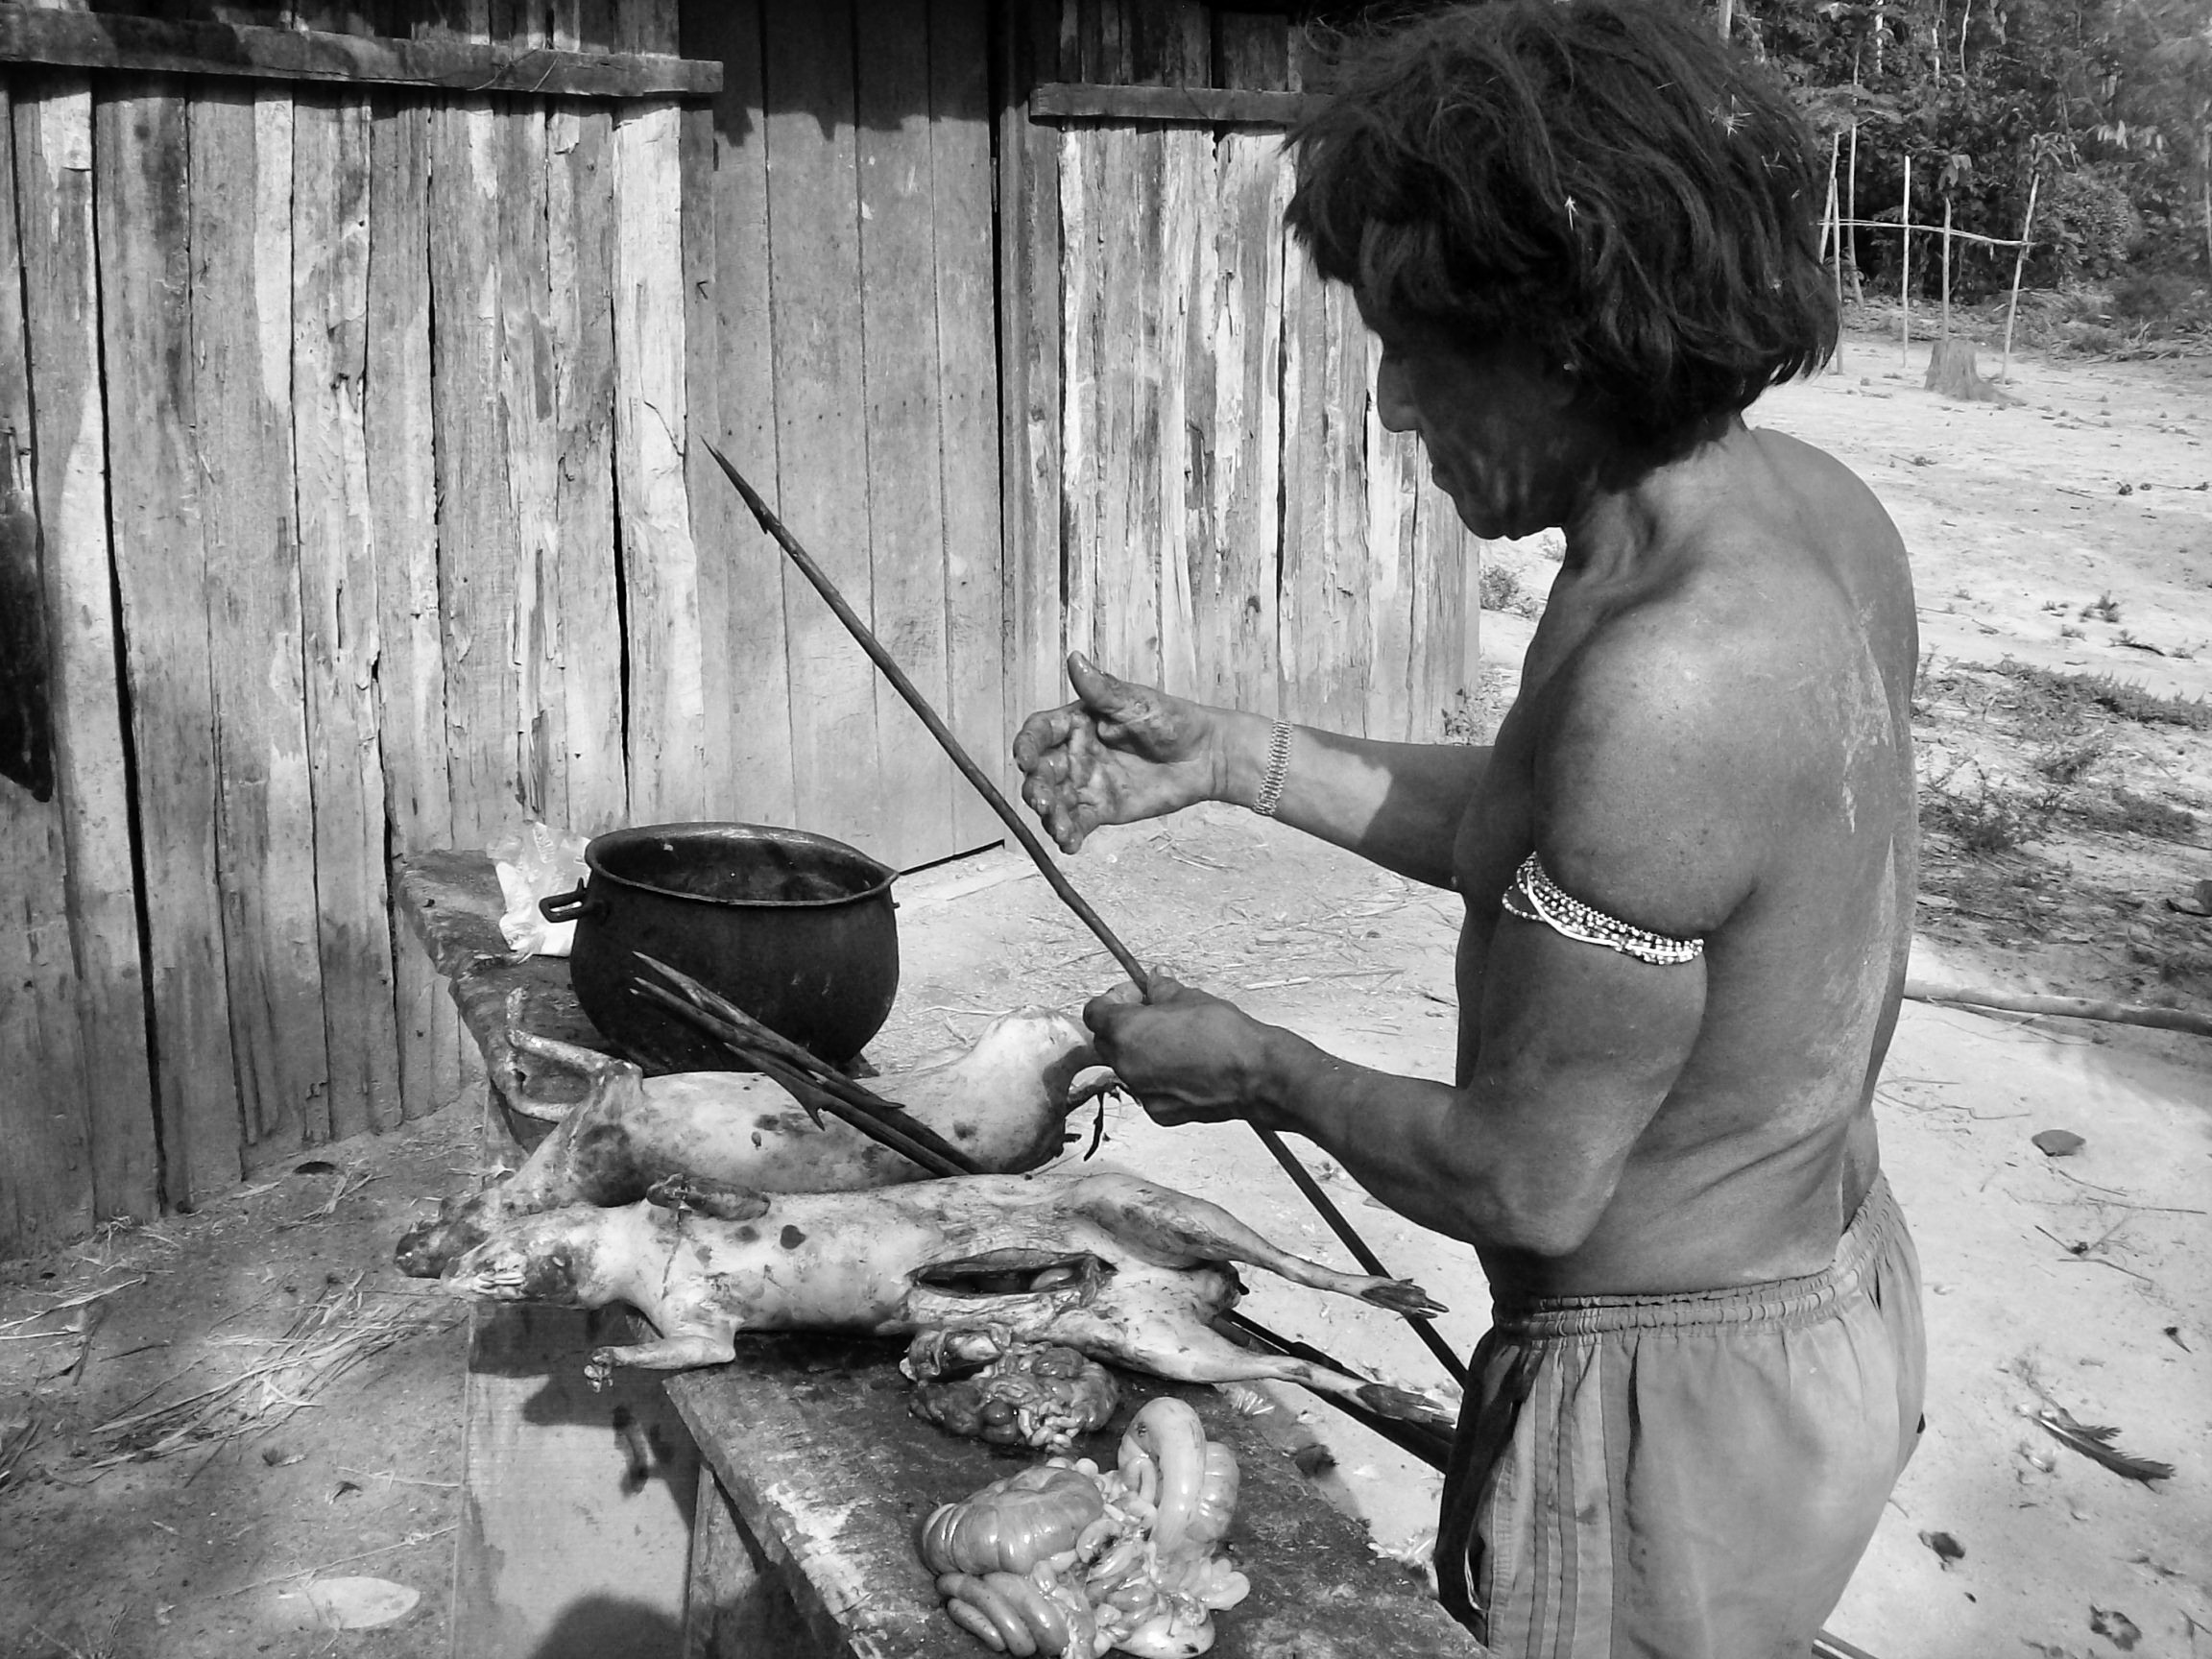
\includegraphics[width=\textwidth]{./imgs/100_5107}
\caption{Kamaraxa’a alimentando as flechas}
\end{figure}

Os Guajá utilizam pelo menos 11 madeiras diferentes para as pontas
dessas flechas menores (\emph{u'ya}). Tais pontas são chamadas
genericamente de \emph{irana'y} (``ponta de pau''), e cada uma delas
remete a algum ser ou elemento que a nomina, um \emph{jara}, um
``dono'', por assim dizer.

\begin{table}[H]
\centering
%\caption{My caption}
\label{my-label}
\begin{tabular}{|l|l|}
\hline
\textbf{Nome da madeira da ponta} & \textbf{Tradução (aproximativa)}                                                              \\ \hline
Ka'i ry'ỹa                        & Ponto do macaco-prego                                                                         \\ \hline
Tapy ry'ya                        & Ponta do rio/água                                                                             \\ \hline
Ka'ihu ny'ỹa                      & Ponta do macaco cairara                                                                       \\ \hline
Maira ry'ỹa                       & Ponta do bagre \emph{maiá}                                                                           \\ \hline
Tapi'i ry'ỹa                      & Ponta da anta                                                                                 \\ \hline
Tamakarõ ny'ỹa                    & Ponta do quatipuru                                                                            \\ \hline
Akwana ny'ỹa                      & Ponta do tucunaré                                                                             \\ \hline
Makari ny'ỹa                      & Ponta do peixe \emph{makari}                                                                         \\ \hline
Tamanawã ny'ỹa                    & Ponta do tamanduá                                                                             \\ \hline
Mata'y                            & Ponta da árvore \emph{mata'y}                                                                        \\ \hline
Aparaty'ỹa                        & \begin{tabular}[c]{@{}l@{}}Ponta não relacionada a \\ nenhum ser, ``apenas pau''\end{tabular} \\ \hline
\end{tabular}
\end{table}

Apesar desta dezena de pontas, as bases tanto de flechas, \emph{wy'ya},
quanto das tabocas, \emph{kĩa}, são basicamente três. Dois tipos de
taquara, chamadas (justamente) \emph{wy'ya} e \emph{iranimu'ya}, além do
filamento central da folha do marajazeiro (\emph{Bactris acanthocarpa}),
também muito dinâmico e resistente, chamado -\emph{ju}. Este último é
utilizado sobretudo na fabricação das tabocas, \emph{kĩa}.

Se por um lado as flechas (\emph{wy'ya}) são projéteis fabricados para
``matar capelães'', por outro as tabocas \emph{kĩa} são os instrumentos
mais letais que os Guajá já produziram. Pira'ima'ã contou"-me que, antes
do contato, um ou outro grupo podia possuir uma panela (\emph{japupua})
velha ou uma faca (\emph{takya}) desgastada. Esses utensílios eram
encontrados, esporadicamente, em acampamentos abandonados --- ou
momentaneamente vazios --- que haviam sido ocupados por madeireiros ou
colonos. Porém, de um modo geral, as ``lâminas'' que utilizavam eram
feitas de tabocas, dentes de paca e cotias, ou mesmo lascas de madeira
mais grossas e resistentes. A taboca foi uma ferramenta de corte e,
durante muito tempo, indispensável aos procedimentos de corte de vários
povos amazônicos. No caso dos Guajá, o bambu"-taboca era lapidado e
amolado pelo preciso dente da paca, transformando"-se numa cortante
lâmina de caça. Era com ela que despelavam as caças, lhes abriam o
ventre e as destripavam --- tudo com essa ``lâmina'' de bambu, bem amolada.
Segundo Wirahoa, a ``faca no mato'' era a taboca. Poucas coisas, com
exceção dos dentes de um queixada e as unhas de uma onça, detinham tanto
poder de cortar (no caso das onças) ou estraçalhar (no caso dos
queixadas) quanto uma taboca (\emph{kĩa}) amolada.

\subsection{Do corte das tabocas}

\forceindent
Um dos verbos utilizados pelos Guajá para se referir a ``cortar'' é
manõ, como no exemplo: \emph{jaha awa ajakara"-manõ ta} ``eu vou cortar o
cabelo das pessoas'' eu + awa + cabelo"-cortar + partícula de aspecto
projetivo (ver Magalhães, \emph{op. cit}., p. 198). Além de \emph{manõ}, o
verbo \emph{kĩxi}, que está associado diretamente ao uso de lâmina, pode
ser usado para `cortar'. Tudo que se relaciona ao corte com facas
amoladas pode ser referido por \emph{tiikĩ}, desde abrir o corpo de um
animal morto até ferir"-se com uma lâmina, dentre outros fatos.
\emph{Tiikĩ} (cortar), \emph{kĩa} (taboca) e \emph{takya} (faca) são
três palavras associadas, cuja tradução literal eu não conseguiria
fornecer, mas que sugerem a taboca (\emph{kĩa}) como um objeto
extremamente cortante: a lâmina por excelência para a tecnologia Guajá.
Nos dias de hoje, algumas pessoas produzem tabocas com pontas de metal,
oriundas de velhos pedaços de faca que são moldados e amolados com limas
até ganharem a forma de uma ponta; essas tabocas também são chamadas
\emph{kĩa}.

Os homens aprendem a confeccionar suas primeiras flechas ainda na
infância. Pais e irmãos mais velhos (e muitas vezes até cunhados)
fabricam pequenas flechas e ensinam as crianças a fazer, a partir de
pequenas ripas de tabocas. Flechas e arcos para as crianças são feitos
com finos pedaços desse bambu, e os meninos as utilizam para matar
lagartos, passarinhos (\emph{iramiria}) e, tal como ocorre a nossas
crianças, as brincadeiras podem ter consequências tragicômicas. O --- à
época --- pequeno Takwaria, por exemplo, foi punido por seu pai e proibido
de utilizar seu pequeno arco e flechinhas, pois no meio de uma
brincadeira atirou propositalmente em seu irmão mais novo causando"-lhe
um pequeno ferimento.

\subsection{Alguns detalhes técnicos}

\forceindent
Após o uso, muitas flechas são reparadas ainda na floresta, quando na
primeira parada ou trégua da caminhada, antes mesmo de voltar para casa.
Da mesma maneira, os cartuchos são preenchidos e recompostos. As avarias
em uma flecha costumam se dar em suas extremidades --- pontas e penas ---,
que podem estar desfeitas, rachadas ou quebradas após o uso. Diante de
qualquer estrago, as pontas, sobretudo, são rapidamente substituídas ou
refeitas. Como veremos adiante, cada flecha é única e, mesmo com tantas
flechas e/ou cartuchos disponíveis, nenhum deles é dispensável.

É certo que todos os homens conseguem fazer boas flechas, porém
enganam"-se os que imaginam que pessoas como os Guajá tenham em cada
homem adulto um especialista completo em todos os ramos da tecnologia de
caça, como se um caçador (seja um caçador exímio ou não) fosse
obrigatoriamente um bom construtor de arcos e flechas; trançador de
fibras; hábil no manuseio de um arco; bom rastreador de caças;
conhecedor dos remédios da floresta e suas curas; dos hábitos animais;
além de cantar e ser versado em cosmologia, xamanismo, etc. Se todos se
interessam por caça e, em média, o fazem muito bem, alguns fabricam
melhor os instrumentos que outros; o mesmo se aplica a outras áreas do
conhecimento. No caso da confecção de um arco, às vezes pode ser difícil
encontrar quem o tenha confeccionado. Tal atividade muitas vezes (tal
como já afirmei) parece também não ter um centro irradiador nem mesmo um
especialista absoluto. Por exemplo, o arco que Pira'ima'ã ``fez'' para me
presentar teve a madeira (\emph{irapara}) retirada por Takya, e a corda,
feita por Hajmakoma'ã. Quando o questionei (com aquela maldade curiosa
presente na relação entre etnógrafo e interlocutores) por que ele não
faria a corda do arco que estava montando para mim --- uma vez que ela
consiste (ao menos eu entendia assim) em quase metade do trabalho de
produzir um arco --- Pira'ima'ã respondeu"-me, tranquilamente, que nunca
aprendera um bom jeito de fazer cordas para arcos tanto quanto
Hajmakoma'ã. E seu pai, ele mesmo um grande trançador, sempre lhe
disponibilizou todas as cordas de que necessitou. Arcos e flechas,
muitas vezes, são feitos a várias mãos. Alguém, a pedido de alguém,
consegue boas taquaras; outro faz as pontas e o corpo; um terceiro tem
uma razoável quantidade de resinas e ceras para os acabamentos; outro
homem possui um estoque razoável de penas; e a esposa, fibras de tucum
(são sempre as esposas que fazem as linhas de tucum). No fim, a flecha
``feita'' por um homem é resultado de um processo que envolve cinco, até
mesmo sete, pessoas diferentes. Isso não significa que as flechas em si,
uma vez feitas, sejam de uso coletivo. Ao contrário, cada um conhece as
suas e só utiliza as que lhe pertencem. O fato é que a forma de
confecção desses artefatos (arcos e flechas) é reflexo do tipo de
economia desempenhada pelos Guajá, a saber, de compartilhamento total da
comida e, como vemos agora, dos serviços e matérias"-primas. E todo o
processo de trabalho acontece de forma muito leve, alegre e, por vezes,
zombeteira.

Redes de troca de bens e serviços, tal como encontramos no Norte (ver
Barbosa, 2007) e Noroeste amazônico (ver Descola, 2006), é algo que os
Guajá praticamente desconhecem. Porém, muitos disseram que antes do
contato era comum trocarem, entre diferentes grupos locais, cocares e
braceletes de pena de tucano, por arcos e flechas; porém não chegava a
se constituir um sistema econômico de troca de bens, tal como ocorre,
por exemplo, nas Guianas (ver Barbosa, \emph{op. cit}.). Aqui não havia grupos
locais que eram exímios e exclusivos fabricantes de flechas, outros que
produziam belos cocares etc., tal a divisão do trabalho que Descola
observa para o piemonte amazônico. O que ocorria aqui era que,
eventualmente, havia um ou outro excelente fazedor de arcos, flechas ou
outro artefato que um grupo local ou outro poderia trocar. Além disso, o
fato de todo homem ter centenas de flechas e alguns poucos arcos, em
média, poderia incentivar essa troca ocasional.

\subsection{\emph{Maka}}

\forceindent
Hoje em dia os Awá caçam os mamíferos terrestres exclusivamente com
espingarda. Porém, ao caçarem macacos, todos acabam tendo chances iguais
(embora a espingarda sempre leve vantagem por sua praticidade e pela
quantidade de chumbos armazenados nos cartuchos que são lançados em um
único tiro). São dois os tipos de cartuchos utilizados: os carregados
industrialmente com chumbo 3T, que os Guajá batizaram de \emph{kaapo} e
chamados ``\emph{3T}'', em português; e os de metal, a que denominam
\emph{jamykera} (``\emph{casca}''), preenchidos pelos homens com pólvora
(\emph{tywerera}), chumbo (\emph{maka'ĩa}), espoletas (\emph{tykyrymyty}
\emph{pykaha}), e selados com cera de abelha, a que se referem em
português por ``\emph{cartucho}'' (se carregado) ou ``\emph{casca}'' (quando
vazio). Os Guajá estabelecem entre os dois tipos de cartuchos a mesma
diferenciação que empregam para as \emph{kĩa} (tabocas) e \emph{wy'ya}
(flechas). Os cartuchos \emph{3T} são mais robustos (próprio a presas
maiores), enquanto os de metal carregados, por serem preenchidos
manualmente --- e pela pressão do chumbo e pólvora ser menor, devido à
camada de cera de abelha ---, ``cospem'' o chumbo com menos propulsão que
os primeiros e se destinam a presas menores. Os cartuchos recarregados
podem até matar caças grandes; porém, uma vez alvejadas, elas conseguem
escapar, devido à menor intensidade do ferimento, e acabam morrendo
longe do local de caça, enquanto que o tiro com o \emph{3T}, devido a
sua força, mata a caça imediatamente. Certa vez, Wirahoa me disse em
português, ``o \emph{3T} é a minha taboca!'', pois com esse cartucho
mataria os mesmos tipos de animais que outrora eram alvejados pelas
tabocas (porcos e antas).

A diferença fundamental entre presas ``grandes'' e ``pequenas'' --- que,
segundo nota Brigthman\footnote{O autor mostra, por exemplo, como entre
  os povos caçadores --- com raríssimas exceções --- as caças maiores são de
  domínio exclusivo das caçadas masculinas; ao passo que as pequenas
  presas podem ser capturadas em caçadas mistas e, muitas vezes,
  exclusivamente por mulheres. Isso nos leva às mesmas questões de
  ``gênero'' que esbocei linhas acima.} (\emph{op. cit}.; baseado em diversos
povos caçadores), se mostra universal quando envolve povos nativos e
predação animal e reverbera em diversas esferas (tecnologia, território,
relações de gênero) --- interessa, em muito, aos Guajá como estamos vendo.
Sua tecnologia de arco e flecha foi transformada pela adoção das
espingardas; porém as ideias que orientam o ato de matar caças grandes
ou caças pequenas continuam embasando as novas tecnologias de caça. Os
problemas são os mesmos, e novas soluções são bem"-vindas.

O barulho das espingardas, apesar de na prática não os incomodar muito,
é algo que os Guajá tematizam, pois ele é resultado do tipo de pólvora
utilizada. As diferentes aldeias se dividem quanto ao uso das pólvoras
brancas e pretas. Na aldeia Juriti, utiliza"-se apenas pólvora branca. É
mais letal, por isso uma pequena quantidade é suficiente para fazer um
grande disparo. Ao passo que as aldeias Tiracambu e \emph{Awá}, até as
últimas vezes em que lá estive, só utilizavam a pólvora preta, menos
letal, mas, por ter que se utilizar em maior quantidade, torna o tiro
dos cartuchos recarregados mais barulhentos (-\emph{po hamãj} ``tiro
grande''). Os caçadores da aldeia Juriti lembram que preferem utilizar a
pólvora branca justamente para fazer seus tiros menos barulhentos. Dizem
que nos primeiros anos muitas pessoas ficavam doentes com o susto pelos
disparos, a alma da pessoa se assustava, \emph{hajtekera pinihĩ}
(``princípio vital assusta"-se''), lembram os Guajá, devido ao tremendo
barulho causado por cada tiro com pólvora preta. O tiro (chamado
-\emph{po}) com a pólvora branca seria parecido com o do rifle, dizem os
Guajá.

\section{Eu, a flecha}\label{eu-a-flecha}

Assim como ocorre aos humanos durante a caçada, as flechas e tabocas
também devem entrar em um estado de ``raiva'' (-\emph{imahy}) para que
funcionem de maneira adequada. Para que desenvolva ``raiva'' é necessário
que os homens lhe forneçam dois elementos cruciais à saúde da flecha:
``dor'' (\emph{hahy}) e ``sangue"-veneno'' (\emph{hawy}). Por isso, após
confeccionada, uma flecha ainda não está pronta para o uso, pois requer
um longo processo de ``alimentação'' e ``envenenamento'' de modo a se
fortalecer e, com isso, aí sim, ser capaz de matar. ``As flechas têm
fome, por isso caçamos muito!'', disse"-me certa vez o velho Takya, um
desses homens que caçam exclusivamente com arco e flechas. Uma flecha se
alimenta fundamentalmente do sangue de suas presas. Uma vez um animal
morto, os homens esfregam na carne cheia de sangue as pontas de diversas
flechas para que, assim, a fome delas seja aplacada. O sangue animal é
dito ``alimento'' (\emph{hami'ũa} --- ``comida dela'') para as flechas, ao
mesmo tempo que é o ``veneno'' (\emph{hawy}) que elas lançarão nas presas
animais. O banho de sangue é a primeira etapa do processo de
transformação da flecha objeto"-em"-si em uma arma mortífera, repleta de
``dor'' e ``raiva'', que será despejada nas presas animais, causando sua
morte. Uma nova flecha, após confeccionada, tem suas pontas revestidas
de sangue e se zanga caso não se a alimente, o que pode fazer com que
não funcione ou que vá contra a vida de uma pessoa; por isso,
fornecem"-lhes o sangue desejado, para que fiquem boas (\emph{katy}).
Certa vez, após uma caçada de macacos, um dos cuxius estava derramando
bastante sangue e, enquanto descansávamos antes de retornarmos à aldeia,
Takya esfregava suas flechas no corpo ensanguentado do animal.

É comum os homens, enquanto estão limpando as caças, levarem junto
algumas flechas para esfregar no corpo do animal após aberto, antes de
destripá"-lo e lavá"-lo. Nessas ocasiões, eles podem, inclusive, conversar
com as flechas, pedindo que elas voltem a matar e que, por isso, as está
alimentando. Os homens também observam que as flechas não param de lhes
pedir sangue. Caso não atendessem a esses incessantes pedidos, elas não
matariam nenhum animal --- se quebrariam ou não acertariam o alvo. Takya
diz que ``conversa'' com suas flechas, pois elas mesmas lhe pedem sangue:
``Me dá \emph{hawykera} (sangue)'', ``eu quero \emph{hawykera}, se você me
der eu terei sangue"-veneno para pegar mais carnes, matar mais bichos. Eu
envenenarei outros animais para você!'' (assim, segundo o velho Takya,
suas flechas falariam). Questionei"-o a respeito de como se dava essa
``comunicação'' entre caçador e flecha. Ele simplesmente respondeu"-me que
é uma coisa que ``os Guajá sabem fazer'' (\emph{awa} \emph{kwa}).

Trata"-se do único uso que fazem do sangue animal, dito extremamente
venenoso (as mulheres não podem sentir sequer o cheiro do sangue de
alguns animais como o veado). Para as flechas, o sangue é como um
remédio (\emph{pohỹ}), enquanto que para os Guajá, ele é um veneno, me
disse certa vez Wirahoa. Devido a tal capacidade letal, ``sangue'' e
``veneno'' são referidos pela mesma palavra na língua Guajá, \emph{hawy};
o veneno de uma cobra é chamado de \emph{hawy}, bem como o sangue que
escorre de uma ferida humana é \emph{hawy}. Em uma taboca se passa o
sangue de animais grandes, como caititu, queixadas e antas, e o desta
última é extremamente benéfico, pois, de maneira mimética, produz na
taboca uma ``dureza'' análoga à do couro de anta: quase indestrutível. Por
outro lado, os animaizinhos pequenos, do tipo que os Guajá não caçam,
como o esquilo caxinguelê (\emph{tamakaja}) ou mesmo ratos
(\emph{awijỹa}), não são possíveis presas na perspectiva de uma flecha.
Certa vez, de forma um tanto irreverente, um homem me afirmou que tais
animais são \emph{maka} \emph{nimá}, \emph{kĩ nima}, e \emph{wy'y}
\emph{nima}, ou seja, animais de criação das espingardas, tabocas e
flechas; por isso as armas não os matam.

As únicas restrições sanguíneas postas a uma flecha são o sangue de uma
onça"-pintada (\emph{jawaruhua}) e o sangue humano (não só dos Guajá, mas
qualquer humano: \emph{awa}, \emph{mihua}, \emph{kamara} ou
\emph{karaia}). O sangue humano é altamente nocivo a uma taboca, e caso
uma dessas flechas venha a matar algum humano ela deve ser imediatamente
descartada, pois corre"-se o risco de uma taboca se acostumar ao sangue
dos humanos e passe a querer sempre mais (voltaremos a esse ponto). Já o
sangue da onça"-pintada (alguns afirmaram) é inapropriado para uma taboca
pois a enfraquece; nesses casos é necessário limpar as ponta da taboca
antes de a colocar novamente em uso --- mas não é necessário descartá"-la.
Essa regra não se aplica à sussuarana (ainda hoje considerada uma
possibilidade alimentar) ou à jaguatirica (que não comem), cujos sangues
também são alimento para as flechas e tabocas. Uma flecha só é jogada
fora caso se quebre, se torne imprestável ou mate um humano.

O sangue, por ser um ``veneno'', atuaria aqui como uma espécie de
\emph{curare}\footnote{\emph{Curare} é um termo genérico que se refere
  aos venenos de caça utilizados por diversos povos ameríndios e, dessa
  forma, ``cobre uma multiplicidade de preparações tóxicas diferentes,
      geralmente à base de plantas do tipo \emph{Strychnos}'' (Descola, 1996:
  309)}, veneno utilizado nas pontas de projéteis de caça por diversos
grupos ameríndios. No caso Ashuar --- um povo que caça com zarabatanas ---
Descola observa que, ao preparar seu \emph{curare} na floresta (entre os
Ashuar é chamado \emph{tseas}), quando cozinham as plantas lentamente,
longe das mulheres e da aldeia, os homens cantam alguns
\emph{anent}\footnote{\emph{Anent} é uma encantação cantada, utilizada
  em todas as circunstâncias da vida cotidiana e ritual Ashuar, a fim de
  alcançar algum resultado desejado ou conquistar os favores de um
  destinatário (Descola, 2006: 495).} para fortalecer o preparado. Tais
encantamentos se dirigem diretamente ao \emph{tseas} (\emph{curare}) de
maneira vocativa, eles lhe ordenam que beba o sangue dos animais contra
os quais será empregado, e cada espécie de caça é nomeada, uma após
outra (Descola, \emph{op. cit.}, p. 310). A fabricação de \emph{curares}, entre
os Ashuar, por exemplo, exige um rigor (distância completa das mulheres;
abstinência sexual; saída da aldeia e reclusão na floresta) que é
ausente no processo de ``envenenamento'' das flechas Guajá. Porém,
enquanto os Jívaro sustentam ser um envenenamento"-encantamento com o
curare durante a preparação das setas da zarabatana --- uma vez que os
encantos \emph{anent} são fundamentais para o bom funcionamento dessas
setas --- os Guajá afirmam que o sangue (\emph{hawy} --- ``sangue"-veneno'')
produz um mesmo envenenamento nas flechas. Muito embora não haja
``encantamento'' (como não há em coisa alguma na vida cotidiana e ritual),
os homens também conversam com suas flechas enquanto as preparam. Essa
conexão entre o sangue consumido e uma boa flecha ocorre mesmo no
aprendizado do manuseio durante a infância. Certa vez o pequeno
Makoraia, que na ocasião tinha apenas cinco anos, atirava em grilos e
calangos que vivem pela área da aldeia e seu entorno as flechinhas
feitas por seu irmão mais velho. Após matar os camaleões, duas de suas
flechas ficaram com a ponta lambuzada de sangue, e ele comentou, rindo,
que deixaria daquele jeito pois é assim que fazem os Guajá.

Quanto ao veneno de caça, a partir de um mito Kachuyana sobre a origem
do curare, (cujo veneno foi dado aos humanos pelo gavião"-real; por isso,
o cipó utilizado por esse povo para o produzir é chamado ``flecha do
gavião"-real''), Lévi"-Strauss argumenta que, nesse caso, o curare,
utilizado basicamente para matar ``macacos coatás'', é besuntado nas
flechas com um pincel de pelos de capelão (Lévi"-Strauss, 2004, p. 315).
Lévi"-Strauss mesmo, indagando o lugar sutil dos venenos de caça nas
culturas ameríndias, indica que ele atua como uma ``intrusão'', uma das
raras situações em que a natureza se aproxima da cultura a ponto de
(quase) determiná"-la. Em uma linguagem musical, os venenos se dispõem em
um (curto) intervalo cromático que --- diferentemente de quase todo
pensamento ameríndio, afeito aos grandes intervalos descontínuos
(diatônicos, portanto) --- faz com que um produto estritamente natural (o
veneno) sirva a uma atividade cultural, a caça (Lévi"-Strauss, \emph{op. cit.},
p. 321. Ver também Descola, 1996, p. 310--311). Penso que podemos incluir
o sangue das flechas Guajá nesse mesmo conjunto, pois, com exceção de
seu envenenamento, o contato com o sangue é evitado em todas as
situações (devido a sua nocividade animalesca). Como se um elemento
pertencente a uma ``extrema'' natureza (diferentemente da carne que é
cozida e consumida enquanto o sangue é lavado e descartado) fosse
desnaturalizado --- ou mesmo culturalizado --- e transformado em veneno.

\begin{center}
***
\end{center}

Após uma flecha ou taboca ser alimentada de sangue"-veneno, ela deve
tornar"-se forte/dura (\emph{hatỹ}). Para isso é posta em um jirau
situado estrategicamente acima do moquém, preso às vigas do teto de um
casa, para que o fogo seque o sangue e a defume (\emph{tataxĩa}). Esse
processo faz com que a flecha assuma uma tonalidade marrom, bem escura
(como pó de café), tendendo para o preto. Quando ela alcança essa cor é
sinal de que está pronta para o uso, capaz de despejar ``veneno'' e ``dor''
em qualquer ser vivente. O objetivo da defumação das flechas é fazer com
que fiquem repletas de \emph{hahy} (dor); é isso que magoa a ferida e
provoca, consequentemente, a morte das presas animais. Como acontece
também com as flechas Yudjá, para os Guajá ``as flechas de caça devem
ser sobredotadas do poder de causar dor: \emph{Sem isso a flecha não
mata nada!''} (Lima 1995, p.110). Tanto a taboca quanto a flecha se
alimentam de sangue, fortalecem"-se com ele; e a fumaça (\emph{tataxĩa}),
além de lhes dar firmeza, as envenena. Uma combinação explosiva.

É importante atentar para a relação entre a fumaça do fogo de cozinha e
os usos benéficos desse elemento. A mesma fumaça que é fundamental no
processamento da carne em alimento (pois a carne é defumada: assada pela
fumaça) endurece e fortalece as flechas (colocando ``dor'' nelas). A
fumaça do fogo de cozinha, dizem os Guajá, retira o sangue dos animais e
endurece a carne para que os humanos possam comer. Ela tem uma função
endurecedora, sendo essa, inclusive, uma das definições de ``culinária''
para os Guajá: o endurecimento da carne e eliminação do sangue. Ao mesmo
tempo que endurece, ela fortalece, e os Guajá imputam tal propriedade à
ação da fumaça. Por exemplo, quando um bebê começa a dar seus primeiros
passos, seus pais e irmãos mais velhos, de forma muito carinhosa,
realizam um procedimento chamado \emph{kytykyty}, ``esfregar'', que
consiste em ``pegar'' a fumaça produzida pela fervura de uma panela, ou da
queima de uma lenha, e esfregar nos joelhos de um bebê, como se
introduzissem a fumaça no corpo da criança para que suas articulações se
enrijeçam (\emph{hatỹ} --- ``ficar duro''), tal como ocorre com a carne
posta a moquear e com a flecha posta a endurecer. Aqui, a fumaça
endureceria as flechas e os ossos (\emph{ikaena})\footnote{Quando se
  está cansado, inclusive, são os ossos (\emph{ikaena}) que estão
  cansados/doloridos, e por isso precisam descansar.}.

O efeito dos projéteis (sejam flechas ou chumbo) sobre os animais,
aquilo que os faz morrer após serem alvejados, se baseia na teoria Guajá
de que tais peças são carregadas de dor (\emph{hahy}) e veneno
(\emph{hawy}). Enquanto o sangue a alimenta, envenenando"-a para que
lance esse veneno em suas presas, é a fumaça que insere \emph{hahy}
(dor) na flecha. Tal procedimento faz com que um animal se fira
gravemente e que a dor e o veneno da flecha sejam transferidos
(``cuspidos'', dizem os Guajá) para ele. Após a presa ser alvejada, a dor
que permanece na ferida (chamada \emph{ha'ina} --- uma espécie de
``bichinho'', me disse um amigo guajá) é que faz o machucado doer,
reforçando a tese de que a dor é sempre externa, algo que é posto de
fora para dentro. Certa vez, alvejaram com espingarda uma cobra surucucu
pico"-de"-jaca (\emph{arikukua}). Abatida instantaneamente, ela foi
``comida pelo chumbo'', um elemento que, tal como as flechas, é faminto
por sangue e portador de muita dor.

O fator complementar (e indispensável) que torna as flechas seres
completamente devastadores e replenos de desejo homicida é a plumagem
escolhida. As penas utilizadas em uma flecha, ainda em sua confecção
inicial, devem ser preferencialmente de aves de rapina (diversas
espécies de gaviões ou harpia) ou mesmo de urubus, porque, de acordo com
a tecnologia Guajá, a plumagem dessas aves tem \emph{hawy}
(sangue"-veneno), já que seus portadores originais se alimentam de carne
e sangue. Para além disso, os Guajá --- de maneira a me traduzir e
simplificar suas ideias --- dizem que os gaviões, por exemplo, aceitam
esse ``acordo'' com os humanos e gostam que suas penas sejam utilizadas
para matar outros animais. Além das penas que gostam de sangue, ainda
utilizam outras excelentes, como de jacu, mutum e até mesmo araras,
embora --- lembro"-me --- prefiram sempre as de gavião (\emph{wiraho}
\emph{popokera} --- ``penas do que foi um gavião''), que por si só são
impregnadas de sangue"-veneno, o que é tão saudável para uma flecha
quanto o sangue espalhado em suas pontas.

É com uma dedicação exemplar que os Guajá cuidam de suas flechas, das
espingardas e da montagem de seus cartuchos. Esses últimos, inclusive,
também se distinguem em relação aos mais preferidos, tal como são as
flechas (umas melhores que as outras). Uma flecha que tenha matado
macacos"-pregos, na caçada seguinte desses animais e após reparada, será
certamente utilizada de novo. E assim sucessivamente. É como se os
objetos fossem se especializando por eles mesmos. Como se a ação do
objeto se manifestasse a partir de sua eficiência. Ao fazer suas
flechas, é comum seu artesão já saber qual será a finalidade de cada
uma, em que animal ele fará com que cada uma se especialize. Certa vez,
o velho Pirama'ã confeccionava suas flechas (\emph{wy'ya}) quando
começou a conversar com Juwi'ia, um de seus netos mais velhos, e lhe
mostrou o que faria com cada uma delas, sugerindo um caráter
exclusivista na utilidade de cada uma. Ele dizia: ``Esta vai para o
capelão, esta outra para o inhambu, esta, para o macaco"-prego, e esta,
para o poraquê'' --- enquanto seu neto (que já era grande) ria e olhava
atentamente, ao mesmo tempo que, para me incluir na conversa, repetia em
português o que o avô estava dizendo. O falecido Pinawãxa'a certa vez
mostrou"-me um cartucho (\emph{jamekera}) que, com ele, havia matado ---
com um único tiro --- dois capelães de uma vez; e teceu vários elogios ao
objeto. Em outra ocasião, Pirama'ã estava caçando capelães e, após
atirar (\emph{japi}) e errar, passou boa parte da tarde procurando pela
flecha usada. ``Era uma boa flecha'' (\emph{wy'ya} \emph{katy}), me disse,
percorrendo uma grande área, até por fim encontrá"-la. Mesmo com centenas
de flechas em seus feixes, uma ``boa flecha'' não pode ser desperdiçada,
pois ela é fruto (muitas vezes) da antiga relação entre si e seu dono
(\emph{jara}).

Para se referir às espingardas e cartuchos, os Guajá recorrem às mesmas
ideias que definem suas flechas, porém, com mais intensidade. Loucas
(\emph{waky}), raivosas (\emph{imahy}), inimigas (\emph{mihua}), dentre
outros adjetivos, servem para definir as espingardas e os cartuchos. Os
cartuchos são ditos incontroláveis. Diferentemente das flechas, eles
matam tudo; até filhotes que se poderiam tomar por animais de criação.
Antes de caçarem com espingardas, matavam"-se muito poucos filhotes
(ainda muito pequenos) de qualquer animal, pois as flechas gostam dos
animaizinhos \emph{nima} (como me disse certa vez Hajmokoma'ã). Por
outro lado, os cartuchos são ``doidos'' e matam tudo. Certa vez, em uma
caçada de capelães havia dois filhotes: um que sobreviveu intacto, e
outro que, alvejado na perna, morreu antes de voltarmos para a aldeia.
Todos disseram que foi o cartucho que o matara; que os cartuchos têm
muito veneno e raiva; e são doidos --- diferentes das flechas, que sabem
(\emph{kwa}) mais.

Outra vez, em uma das reuniões com membros do \versal{CGIIRC}, quando os Guajá
discutiam a necessidade de uma política a favor da compra e manutenção
de armas de fogo --- frente ao Estatuto do Desarmamento brasileiro, que a
Funai aplica desde a Lei Nº 10.826 de 2003 quando se instituiu o Sistema
Nacional de Armas no Brasil\footnote{Cf. \emph{www.planalto.gov.br/ccivil\_03/leis/2003/L10.826.htm},
  acesso em 27/01/2016. Um problema central em todas as aldeias é a
  falta clara de uma política para a compra de munição e a manutenção
  das armas de fogo entre este povo, cuja subsistência e economia
  simbólica é dependente da caça. De tempos em tempos seu debate volta à
  tona, com imagens que evocam um ``faroeste''; sugerindo que os
  indígenas não teriam a competência ou preparo psicológico para
  utilizar armas de fogo. Visto que esses povos são, grosso modo,
  considerados um empecilho ao desenvolvimento, capazes de atacar
  colonos e frear o avanço da fronteira com seus arcos, flechas e
  bordunas, o uso de espingardas torná-los"-ia ainda mais perigosos. Para
  outros, a introdução de novas tecnologias nas comunidades indígenas os
  ``viciariam'' ao ponto de incentivá-los a abrir mão de seus
  conhecimentos tradicionais, além de propiciar o rápido esgotamento dos
  recursos naturais em suas áreas. Não compartilho com nenhuma das duas
  posições, defendo que para um povo como os Guajá, a partir de uma
  série de pontos e reflexões que estamos vendo no decorrer deste livro,
  a caça com armas de fogo é uma alternativa sustentável e indispensável
  à vida deles, dado o ganho econômico oriundo de sua utilização.} ---; ao
tentar convencê"-los dos perigos de caçar com espingarda, um
representante da Funai argumentou que as armas, além de tudo, eram
perigosas, pois as pessoas eventualmente podem matar umas às outras com
elas, e os brancos (\emph{karaia}), que se matam com armas, são a melhor
prova disso. Um dos representantes guajá fez então uma breve fala;
lembrou que os brancos só morrem nas mãos das armas de fogo porque
atiram um nos outros com elas, e que os Guajá, por não atirarem flechas
uns nos outros, não morrem pela flecha, e muito menos isso aconteceria
com as armas de fogo. Lembrou também que o uso que fazem de arma de fogo
é, por incrível que possa parecer, ainda menos letal que o uso que fazem
das flechas. Esse jovem líder, chamado Itaxĩa, enumerou um razoável
conjunto de casos de pessoas que haviam sido atingidas por flechas
desgovernadas ou que caíam no lugar errado, enquanto que com as armas de
fogo acidentes como esse nunca aconteciam. Em poucas palavras, de forma
perspicaz --- ao menos para mim --- Itaxĩa estava argumentando que, da
maneira que os guajá utilizam suas armas de fogo, elas são menos
perigosas do que flechas e tabocas.

A crise que os Guajá enfrentam hoje, pela falta de munição é concebida
por eles como fruto de uma esquizofrenia política do estado brasileiro,
em particular, da Funai. Todos conseguem relembrar a chegada das
espingardas nas aldeias: do barulho, o estranhamento, o cheiro de
pólvora e, sobretudo, o rendimento econômico que essa nova tecnologia
proporcionou à ``boa vida'' (\emph{iku katy}) humana. As chamadas
``\emph{Vinte}'' (espingarda de calibre 20) entraram na caça Guajá logo
nos primeiros dias de contato, porém hoje as pessoas não podem comprar
munição, muito menos novas espingardas, pois é proibido por lei. Os
Guajá não entendem por que foram convencidos a escolher a espingarda no
lugar de suas flechas há poucas décadas, ficando completamente
dependentes da caça com armas de fogo, e a mesma Funai que lhes
possibilitou essa transição diz que não podem mais possuir suas armas
nem comprar a munição.

\begin{center}
***
\end{center}

Passar sangue nas flechas, como estamos vendo, é um processo alimentar e
de envenenamento. Hoje, os Guajá chamam essa operação de ``lustrar'' (em
português). Da mesma forma que lustram suas espingardas com o óleo de
máquina, lustram suas flechas com sangue. Tal como uma flecha tem fome
de sangue, uma espingarda (\emph{maka}) tem fome de óleo. O ato de
lustrar a espingarda parece produzir na arma um efeito análogo ao
alcançado quando lustram as flechas com sangue. Assim, para a arma, o
óleo produz o mesmo efeito alimentar que o sangue produz nas flechas,
fazendo com que fique forte e com raiva, ao mesmo tempo que aplaca sua
fome. Lembro"-me de, nos meus primeiros dias na aldeia Juriti, reparar
que todos os homens passavam boa parte do dia desmontando as
espingardas, até suas mínimas peças, e tornavam a montar, as limpavam e
lustravam. Isto ocorria quase que diariamente, da mesma forma que os
velhos fazem com as flechas; não só as reparam, mas também as alimentam
e criam (\emph{riku}), como garantem ser a relação de um caçador e sua
flecha (voltaremos a esse ponto).

De tanto montar e desmontar, as armas são repletas de remendos e
adaptações e constantemente voltam a quebrar. Muitas vezes os defeitos
são provocados por essa extrema manutenção diária, e não pelo uso
intenso, propriamente. Isso gera comentários infelizes por parte de
alguns funcionários do Posto Indígena, em um jogo de ataques e defesas
entre os próprios funcionários. Alguns criticam que os homens são
incapazes de possuir uma espingarda sem as quebrar ou que as armas só se
quebram porque ``mexem'' muito nelas. Outros os defendem, dizendo que as
espingardas se quebram porque seu uso é o ``ganha"-pão'' deles; que eles
precisam utilizá"-las muito mais do que os ``brancos'', e por isso elas se
quebrariam tanto. O fato é que há uma total dependência dos Guajá em
relação à Funai para a compra de munição e o reparo das espingardas
(quando precisam de reposição de peças) --- o que nem sempre dá certo. A
maior parte de minhas reservas financeiras foram repassadas para comprar
munição (artigo muito caro) e pagar reparos de espingardas, a pedido dos
Guajá ou dos próprios funcionários da Funai (no caso do reparo de
espingardas, funcionários chegavam a me pedir ajuda, pois a
administração da Funai dificilmente paga reparos). Com suas espingardas
quebradas, os homens ficam muito apreensivos, pegam emprestadas as armas
de seus irmãos que, devido ao uso intenso, também podem se quebrar. E
isso seria uma espingarda a menos na aldeia. As espingardas (e
principalmente a munição) são o principal assunto entre os homens e os
funcionários do posto. Para estes, os Guajá utilizam mal a espingarda,
para os Guajá, os funcionários são sovinas, pois teriam acesso a uma
grande quantidade de munição com os \emph{karaia} das cidades, mas
regulam e não a fornecem na quantidade adequada\footnote{Só para termos
  uma ideia, a munição foi a única exigência colocada pelos Guajá de
  todas as aldeias, quando solicitei autorização de pesquisa à Funai. Em
  2007, ao chegar pela primeira vez na aldeia Juriti, por ter comprado a
  munição na companhia de um funcionário da Funai ele pediu"-me que a
  deixasse com ele, pois os Guajá ainda tinham um pouco em suas casas, e
  se eu distribuísse tudo de uma só vez eles a consumiriam rapidamente.
  Argumentei então que daria ao menos uma parte para que as pessoas
  vissem que eu havia trazido o que elas me pediram. Foi o que fiz, sem
  maiores problemas. Ao me perguntarem se eu havia trazido mais do que
  aquela pequena quantidade que distribuía, informei"-lhes que o chefe de
  posto havia retido uma parte da munição que eu havia levado para lhes
  dar em outra ocasião, quando precisassem novamente. Com isso, ficaram
  chateados comigo dizendo que, da próxima vez que eu os visitasse,
  desse toda a munição a eles, diretamente. Assim o fiz na minha segunda
  viagem, em 2008. Ao retornar à aldeia Juriti, comuniquei ao chefe do
  Posto que entregaria a munição diretamente aos homens, pois eles assim
  haviam me pedido. Um pouco contrariado, o funcionário aceitou minha
  proposta. Ao distribuir a munição aos homens eles me pediram que eu
  desse somente metade a eles e entregasse a outra metade ao chefe de
  posto, para que ele guardasse melhor e depois distribuísse mais um
  pouco. Eu insisti que não, que pegassem tudo, pois seria melhor para
  eles. No entanto, me asseguraram que ainda tinham alguma munição
  guardada em suas casas e que, por isso, era melhor armazenar esse
  excedente na sede do posto. Quando precisassem, solicitariam ao chefe
  de Posto.}.

Além do óleo, os homens me pediam que comprasse tinta de metal da cor
preta para pintarem os canos e as partes de metal de suas espingardas.
Segundo me explicou Wirahoa --- nessa teoria Guajá sobre as armas (e o
metal) ---, o cano da espingarda (originalmente metálico ou dourado),
estando na cor preta, ``enxergaria'' melhor a caça, tal como ocorre com as
flechas ``defumadas'' que, enegrecidas, aguçam sua ``visão'' e potência.
Como vimos, após sangradas e defumadas, as flechas ficam escuras, como
se fossem queimadas, e por não poderem fazer o mesmo com a espingarda
(deixar em cima de um moquém), pois a estragariam; a tinta preta
produziria o mesmo efeito, faria com que ela se tornasse mais eficiente.

\section{Objetos inimigos são domesticados}

As tabocas e as flechas são ditas serem \emph{mihua} (``inimigas'',
``selvagens'') que, como vimos, é também o termo pelo qual classificam
diversos grupos distantes, com os quais mantêm relações de inimizade em
potencial, os ``Guajá brabos'', como costumam dizer. Wirahoa diz que no
processo comunicacional entre as flechas e seus donos elas falam: ``Me
coloque no fogo quente!\ldots{} Isso mesmo, mais quente, mais quente!\ldots{} e
agora me levem para matar porcos''. Por isso, se forem bem defumadas
matarão suas presas animais com mais facilidade, como se seu
veneno"-sangue (\emph{hawy}) estivesse muito ativo. Ainda segundo
Wirahoa, quando uma flecha está no arco, prestes a ser atirada
(-\emph{japi}), é como se ela dissesse ao animal: ``Eu sou \emph{mihua}
(`braba'), não sou seu \emph{harapihiara} (cognato, parente próximo),
não sou sua amiga (\emph{aty}) eu só gosto dos \emph{awa} (humanos),
pois eles cuidam de mim (\emph{riku}), me alimentam\ldots{} por isso eu vou
te matar!'' Portanto, as flechas são inimigas, criadas para serem assim.
Mas, por serem domesticadas pelos humanos, mesmo sendo ``brabas'' quase
nunca os atacam, ao contrário do que ocorre com o chumbo
(\emph{maka'ina}) dos cartuchos (\emph{jamekera}), que não obedecem a
ninguém, são ``doidos'' (\emph{waky}).

Vimos no capítulo anterior que os Guajá desenvolveram uma forma de
anulação da distância cognática (se assim podemos pensar) a partir da
ideia"-relação \emph{riku}. Da mesma maneira que o \emph{riku} funciona
entre diversos seres, os muitos agenciamentos entre um caçador e suas
flechas e tabocas são da ordem de uma relação \emph{riku}. Fabricá"-las é
só um primeiro passo para as possuir. E ninguém possui uma flecha só
porque a fabricou, pois possuí"-las é obrigatoriamente ``criá"-las''
(\emph{riku}). Muito embora essas armas de caça e guerra sejam feitas
(como objetos) pelos humanos, têm uma autonomia a ponto de seus donos
manterem com elas uma relação \emph{riku}. Em outras palavras, como
sempre me foi traduzido, os homens ``criam'' suas flechas, e criá"-las
implica basicamente confeccioná"-las (obviamente, porém com as penas
certas), alimentá"-las e repará"-las sempre que necessário --- um processo
constante e de longa duração. Por serem perigosas (\emph{mihua}),
somente a domesticação (\emph{riku}) pode lhes proporcionar uma vida
proveitosa (sem acidentes e tragédias), sendo que parte da destreza do
caçador está na qualidade dessa relação estabelecida com seu feixe de
flechas. As flechas e tabocas agem intencionalmente: se não desejarem
funcionar não funcionam (quebram, erram o alvo, se perdem). Por isso
elas estão no \emph{hall} dos ``seres domesticáveis''. Por agir com
intenção e vontade, algumas flechas e tabocas se prestam a matar alguns
animais de forma mais eficiente do que outras, e algumas delas são
excelentes companheiras de caça. Em seu arsenal domiciliar, aqueles
homens que não fazem uso de espingarda contam, em média, com 200
projéteis, entre flechas e tabocas.

Quando saem para a mata, carregam de 15 a 30 projéteis formados em um
feixe, precisamente amarrados por um cipó e com as pontas em conjunto
envoltas por uma folha larga de palmeira, tal como uma delicada
embalagem protetora. Esse cuidado se justifica, pois garante que as
pontas afiadas não trisquem em nada e não sejam avariadas durante as
longas caminhadas. Firmeza, retidão, fio adequado, dentre tantos fatores
técnicos, são levados em conta para que uma flecha esteja o mais próximo
da perfeição. O velho Pirama'ã, um exímio arqueiro, uma vez na mata,
antes de subir numa árvore atrás de capelães ou se embrenhar por um
brejo à procura de um poraquê, seleciona, de seu feixe, as flechas que
realmente lhe serão úteis: morde"-as, entorta"-as, confere a plumagem e\ldots{}
conversa com elas: tarefas importantes, feitas com concentração. No
entanto, como quase tudo na vida cotidiana dos Guajá, essas ações
ocorrem sem nenhum cerimonialismo. Ele apenas deve se certificar de que
são as flechas certas para ``estar com'' ele (\emph{riku}). As flechas são
aproveitadas até se esgotarem. Só são descartadas quando se quebram
completamente.

Embora eu não tenha coletado nenhum mito específico sobre a origem das
flechas e seus usos, sei que, para os Guajá, \emph{Maíra} possuía
flechas mágicas que, ao invés de tirar, davam vida aos seres. Como
exemplo, após \emph{Maíra} ter transformado uma pedra na primeira anta
(\emph{tapi'ira}), ele atirou uma de suas flechas na anta"-pedra e ela
saiu correndo na forma de anta; e quando transformou um cupinzeiro no
primeiro queixada fez o mesmo. Há, na verdade, duas interpretações para
o procedimento de \emph{Maíra} nesses feitos magníficos. Um é que ele
apenas gritou ``Vá, anta!'' (\emph{awyhy!}, ``corra''); e o outro ao atirar
flechas mágicas, também gritando ``Vá, anta!'' Com exceção de episódios
como esse (ver anexo de mitos), não encontrei na mitologia guajá
histórias específicas sobre flechas. No entanto, a mitologia ameríndia é
repleta de episódios que as apresentam como seres"-objetos repletos de
desejo, intenção e autonomia: flechas especializadas em caças
específicas e mesmo algumas que caçam sozinhas estão presentes, de uma
forma geral (no último capítulo, veremos como são as flechas dos
\emph{karawara}, energizadas, com que caçam na Terra). Há um mito
Karajá, apresentado por Lévi Strauss (\versal{M}177), sobre um caçador que obtém
a proteção de uma rã em troca de carícias ilusórias e que se torna ``um
caçador milagroso, graças a zagaias dadas por ela (a rã), `uma para
cada tipo de alimento', cuja força é preciso atenuar
besuntando"-as com um unguento, que equivale, portanto, a uma espécie de
veneno de caça invertido'' (Lévi"-Strauss, 2004, p. 197). Veremos adiante
como os \emph{karawara}, de alguma forma, representam um certo ideal de
caça guajá que prescreve tal exclusividade: de um tipo de caçador para
um tipo de caça, tal como uma flecha específica para uma caça específica
--- como quis mostrar"-me Pirama'ã (relacionando suas flechas aos animais
que elas preferencialmente vão matar) e como encontramos na mitologia
ameríndia (ver \versal{M}177 em Lévi"-Strauss, 2004, p. 197).

Em outros casos analisados por Lévi"-Strauss, em dois mitos Toba (\versal{M}212 e
\versal{M}213), sobre a ``moça louca por mel'', há uma referência a ``flechas
mágicas'' lançadas por um pica"-pau que, ao notar o sumiço de sua esposa,
dispara"-as em várias direções para que procurem a mulher desaparecida.
As flechas não obtêm sucesso e voltam sozinhas até seu dono, assim, ele
percebe que sua mulher não foi encontrada por suas flechas (em uma das
versões, \versal{M}212, uma flecha a encontra e as outras retornam ao dono). Há
outros mitos sobre flechas muito precisas, que conseguem acertar o meio
de um fino cipó; ou ainda, se lançadas ao alto, ao cair acertam em cheio
o dorso de um animal; dentre outras. Há ainda um mito Waiãpi, coletado
por Gallois (1988), sobre a origem das flechas e dos acidentes com
flechas que sustenta que, antigamente, quando os caçadores lançavam suas
flechas, eles diziam a elas: ``volte flecha, pode voltar''. Eis que as
flechas falavam: ``cuidado, se afaste eu vou descer''. Hoje, as flechas
não falam mais e podem acertar qualquer um. Isto posto, da mesma forma
os Guajá gostam de pensar que cada uma de suas flechas tem predileção
especial por determinado animal, nunca falado de forma explícita, mas na
prática eles selecionam flechas com ``histórico'' de predações
específicas. Pois, uma flecha que já matou muitos macacos"-pregos
continuará sendo utilizada para matar macacos"-pregos; e assim
sucessivamente, como se a ação fosse imanente ao objeto, independente do
caçador.

Para finalizar este capítulo, em que busquei descrever aspectos técnicos
das atividades de caça, lembro que se a mesma taboca que assassinou um
humano for reutilizada em outra caçada, tempos depois, ela certamente
desprezará o alvo e se voltará contra aqueles que estiverem ao redor do
caçador, em busca de mais sangue humano. Por isso, uma taboca que já
experimentou desse sangue deve ser inutilizada\footnote{Isso faz lembrar
  o citado mito Karajá (\versal{M}177, Lévi"-Strauss, 2004a: 353) em que o caçador
  consegue flechas mágicas para destruir ``uma raça de macacos canibais,
  da espécie guariba'', porém as flechas são tão venenosas que o caçador
  precisa enfraquecê"-las (desenvenená"-las) com o tal unguento mágico
  pois, caso contrário, ela se voltaria contra o próprio caçador.}. Algo
semelhante ocorre com o próprio matador de guerra Guajá (bem como outros
casos Tupi), que aqui absorve a raiva (\emph{ha'aera}) (não o sangue) do
inimigo e se torna perigoso à vida na aldeia, um quase"-inimigo (como
sabemos, a partir também do já clássico caso Araweté, Viveiros de Castro
1986). Por isso, tanto um matador quanto uma taboca assassina
representam ambos uma ameaça real para toda a vida da aldeia e, por
segurança, a taboca que se alimentou de sangue humano deve ser
descartada, enquanto quem matou cumpre um resguardo.

Devo aqui lembrar que na Amazônia a taboca é parte constituinte (e
central) de muitos arsenais de guerra; peça"-chave em diversos contextos,
sendo que para alguns grupos (como os Jívaro) eram armas exclusivas de
guerra, e não de caça. Desta forma, de acordo com meus interlocutores,
as tabocas (\emph{kĩa}) têm uma especial predileção por sangue humano,
pois são ``naturalmente'' propensas a gostar dessa qualidade de sangue, já
que foram criadas para comer/matar os inimigos humanos (além, é claro,
dos animais de grande porte). Por isso, caso uma taboca mate um humano,
ela quererá envenenar (ou, ao menos, ferir) outros humanos com esse
sangue; pois fica \emph{doida} (\emph{waky}) e tudo fará a fim de
experimentar novamente tal sangue enlouquecedor\footnote{A relação entre
  o sangue e a loucura é mais uma variação da relação entre sangue e
  doença, como já foi mencionado. Além do sangue humano, não consomem um
  tipo de jacu, pois o sangue desse animal os enlouquece (na verdade,
  provoca ataques epiléticos) --- ``tal como a cachaça faz com Guajajara'',
  me disseram.}. A flecha deve ser descartada no mato, pois ela é agora
uma matadora de humanos e vai querer o sangue de outros Guajá. Não se
quebra uma taboca, apenas joga"-se fora.

Sabemos que um guerreiro homicida Araweté é aquele que mata (ou flecha)
um inimigo em conflito e cuja barriga está, por isso, cheia de sangue
(que deve ser vomitado e expelido), transformando esse guerreiro também
em um íntimo e temporário inimigo, além de uma pessoa psicológica e
permanentemente instável. Assim, ele permanecerá para sempre
meio"-inimigo, volúvel, propenso a rompantes de ciúme, violência, e mesmo
homicídio, ainda que entre os seus --- independentemente do que faça para
se livrar dessa condição (Viveiros de Castro, 1986, p. 594). Do mesmo
modo, as tabocas assassinas Guajá também se tornam inimigas, algo que em
potência sempre foram e que, após um homicídio, se torna irreversível.
Isso se dá porque, tal como para o homicida Tupi, a taboca (\emph{kĩa})
Guajá penetra na carne e se alimenta do sangue de um inimigo, passando
por um processo análogo ao do guerreiro Araweté, transformando"-se em
\emph{mihua}, ``inimiga'', dizem os Guajá. O matador Araweté se torna um
inimigo, ``um devir"-outro do guerreiro, uma traição à sociedade''
(Viveiros de Castro, 1986, p. 593), cujo armamento deve ser dele
afastado, pois, ``sedento de vingança, inspira seu matador a um furor,
uma vontade cega de prosseguir matando'' (\emph{idem}), mesmo que isso implique
matar parentes. Com alguns reparos, podemos afirmar o mesmo para a
taboca Guajá, ela é uma ``traição'' a quem a fabricou, pois pode se
voltar, inclusive, contra seu dono.

Assim é a taboca que experimenta o sangue humano. Ao ser reutilizada em
uma caçada, quando for atirada (\emph{japi}) poderá escapar e matar
qualquer pessoa de um grupo de caça, tudo isso ``intencionalmente'',
porque deseja matar de novo. Porém, por mais \emph{atitude} que os Guajá
possam atribuir a uma taboca, ela (ainda) é um objeto, que pode (e deve,
nesses casos) ser descartado e substituído, tal como fazemos com
qualquer outro objeto. Não se destrói uma ``taboca doida'' (\emph{waky}
\emph{kĩa}). Ela é simplesmente abandonada, devoluta. Não entendo o
porquê, mas os Guajá afirmaram que ela não pode ser quebrada; somente
jogada fora, no mato, tal como um corpo inimigo é abandonado após um
homicídio. Se na Amazônia indígena animais e objetos podem ser
``pessoas'', eles o serão até o fim.

Por fim, mesmo sendo criadas e cuidadas, as flechas não contam com
nenhum tipo de cuidado específico ou cerimonial; nenhuma evitação. Até
as mulheres as manuseiam e eventualmente as utilizam como lanças em suas
caçadas (sem atirá"-las com o arco, é certo). Certa vez, ao cozinhar em
uma panela, o jovem Juxa'a estava mexendo na água do cozido e pegando
pedaços de carnes, com o auxílio de uma flecha que estava ao seu
alcance. Utilizou a flecha como um garfo; e não se tratava de uma peça
velha, que estivesse fora de uso, mas de uma ``boa flecha'' (\emph{katy}).
Isto não quer dizer que as flechas recebam um cuidado ordinário. Ao
contrário, elas são tratadas com muito esmero. Mesmo com tal
desprendimento (correlato a toda ausência cerimonial que conduz a boa
vida dos guajá) --- e diferentemente de quase todos os outros objetos
vulgares que existem espalhados pelo chão da aldeia Juriti (sapatos,
roupas, panelas, talheres, crânios de animais, cachos secos de fruto,
ferramentas, dentre tantas outras coisas), cobertos de pó e sujeira ---,
as flechas nunca são negligenciadas. Se forem velhas, as recuperam ou as
deixam no mato (ou em qualquer lugar), perdidas ou abandonadas, para que
``morram'' sozinhas.
